
% options:
% thesis=B bachelor's thesis
% thesis=M master's thesis
% czech thesis in Czech language
% english thesis in English language
% hidelinks remove colour boxes around hyperlinks

\documentclass[thesis=M,english]{FITthesis}[2012/10/20]

% \usepackage[utf8]{inputenc} % LaTeX source encoded as UTF-8
% \usepackage[latin2]{inputenc} % LaTeX source encoded as ISO-8859-2
% \usepackage[cp1250]{inputenc} % LaTeX source encoded as Windows-1250

\usepackage{graphicx} %graphics files inclusion
%\usepackage{subfig}
\usepackage{amsmath}
\usepackage{amssymb}
\usepackage[chapter]{algorithm} % http://ctan.org/pkg/algorithms
\usepackage[noend]{algpseudocode} % http://ctan.org/pkg/algorithmicx
\usepackage{pseudocode}
\usepackage{comment}
\usepackage{enumitem}
\usepackage{amssymb}
\usepackage{caption}
\usepackage{subcaption}
\usepackage[section]{placeins}

\usepackage{dirtree} %directory tree visualisation

% % list of acronyms
% \usepackage[acronym,nonumberlist,toc,numberedsection=autolabel]{glossaries}
% \iflanguage{czech}{\renewcommand*{\acronymname}{Seznam pou{\v z}it{\' y}ch zkratek}}{}
% \makeglossaries

%%%%%%%%%%%% own commands %%%%%%%%%%%%%%%%%%
\newcommand{\matr}[1]{\mathbf{#1}} 
\newcommand{\argmax}{\mathop{\mathrm{argmax}}}

\makeatletter
\def\BState{\State\hskip-\ALG@thistlm}
\makeatother
%\newcommand{\max}{\mathop{\mathrm{max}}}

% % % % % % % % % % % % % % % % % % % % % % % % % % % % % % 
% EDIT THIS
% % % % % % % % % % % % % % % % % % % % % % % % % % % % % % 

\department{Department of Theoretical Computer Science }
\title{Thesis title (SPECIFY)}
\authorGN{Luk{\' a}{\v s}} %author's given name/names
\authorFN{Lopatovsk{\' y}} %author's surname
\author{Luk{\' a}{\v s} Lopatovsk{\' y}} %author's name without academic degrees
\authorWithDegrees{Bc. Luk{\' a}{\v s} Lopatovsk{\' y}} %author's name with academic degrees
\supervisor{Ing. Daniel Va{v s}ata, Ph.D.}
\acknowledgements{THANKS (remove entirely in case you do not with to thank anyone)}
\abstractEN{Summarize the contents and contribution of your work in a few sentences in English language.}
\abstractCS{V n{\v e}kolika v{\v e}t{\' a}ch shr{\v n}te obsah a p{\v r}{\' i}nos t{\' e}to pr{\' a}ce v {\v c}esk{\' e}m jazyce.}
\placeForDeclarationOfAuthenticity{Prague}
\keywordsCS{Replace with comma-separated list of keywords in Czech.}
\keywordsEN{HMM, CT-HMM.}
\declarationOfAuthenticityOption{1} %select as appropriate, according to the desired license (integer 1-6)
% \website{http://site.example/thesis} %optional thesis URL


\begin{document}

% \newacronym{CVUT}{{\v C}VUT}{{\v C}esk{\' e} vysok{\' e} u{\v c}en{\' i} technick{\' e} v Praze}
% \newacronym{FIT}{FIT}{Fakulta informa{\v c}n{\' i}ch technologi{\' i}}

\setsecnumdepth{part}

\begin{introduction}
	This is the master thesis. welcome!
	\section{Motivation and objectives}
	About a discrete model [inspired by Rabiner? ] and why it is not satisfactory  %(as http://delivery.acm.org/10.1145/350000/343402/p162-aziz.pdf?ip=147.32.98.33&id=343402&acc=ACTIVE%20SERVICE&key=D6C3EEB3AD96C931%2E9BD1EC80ACA8C1C5%2E4D4702B0C3E38B35%2E4D4702B0C3E38B35&CFID=702042173&CFTOKEN=62280276&__acm__=1481276923_1a71eb623e1c42d4c8e9b84178eb248f)	
	Add articles and DP that have done it before - less or more successfully 
	
The figure example \ref{fig:gb}.

CT-HMM is the natural extension of discrete-time model, that ..


\begin{figure}[h]
\centering
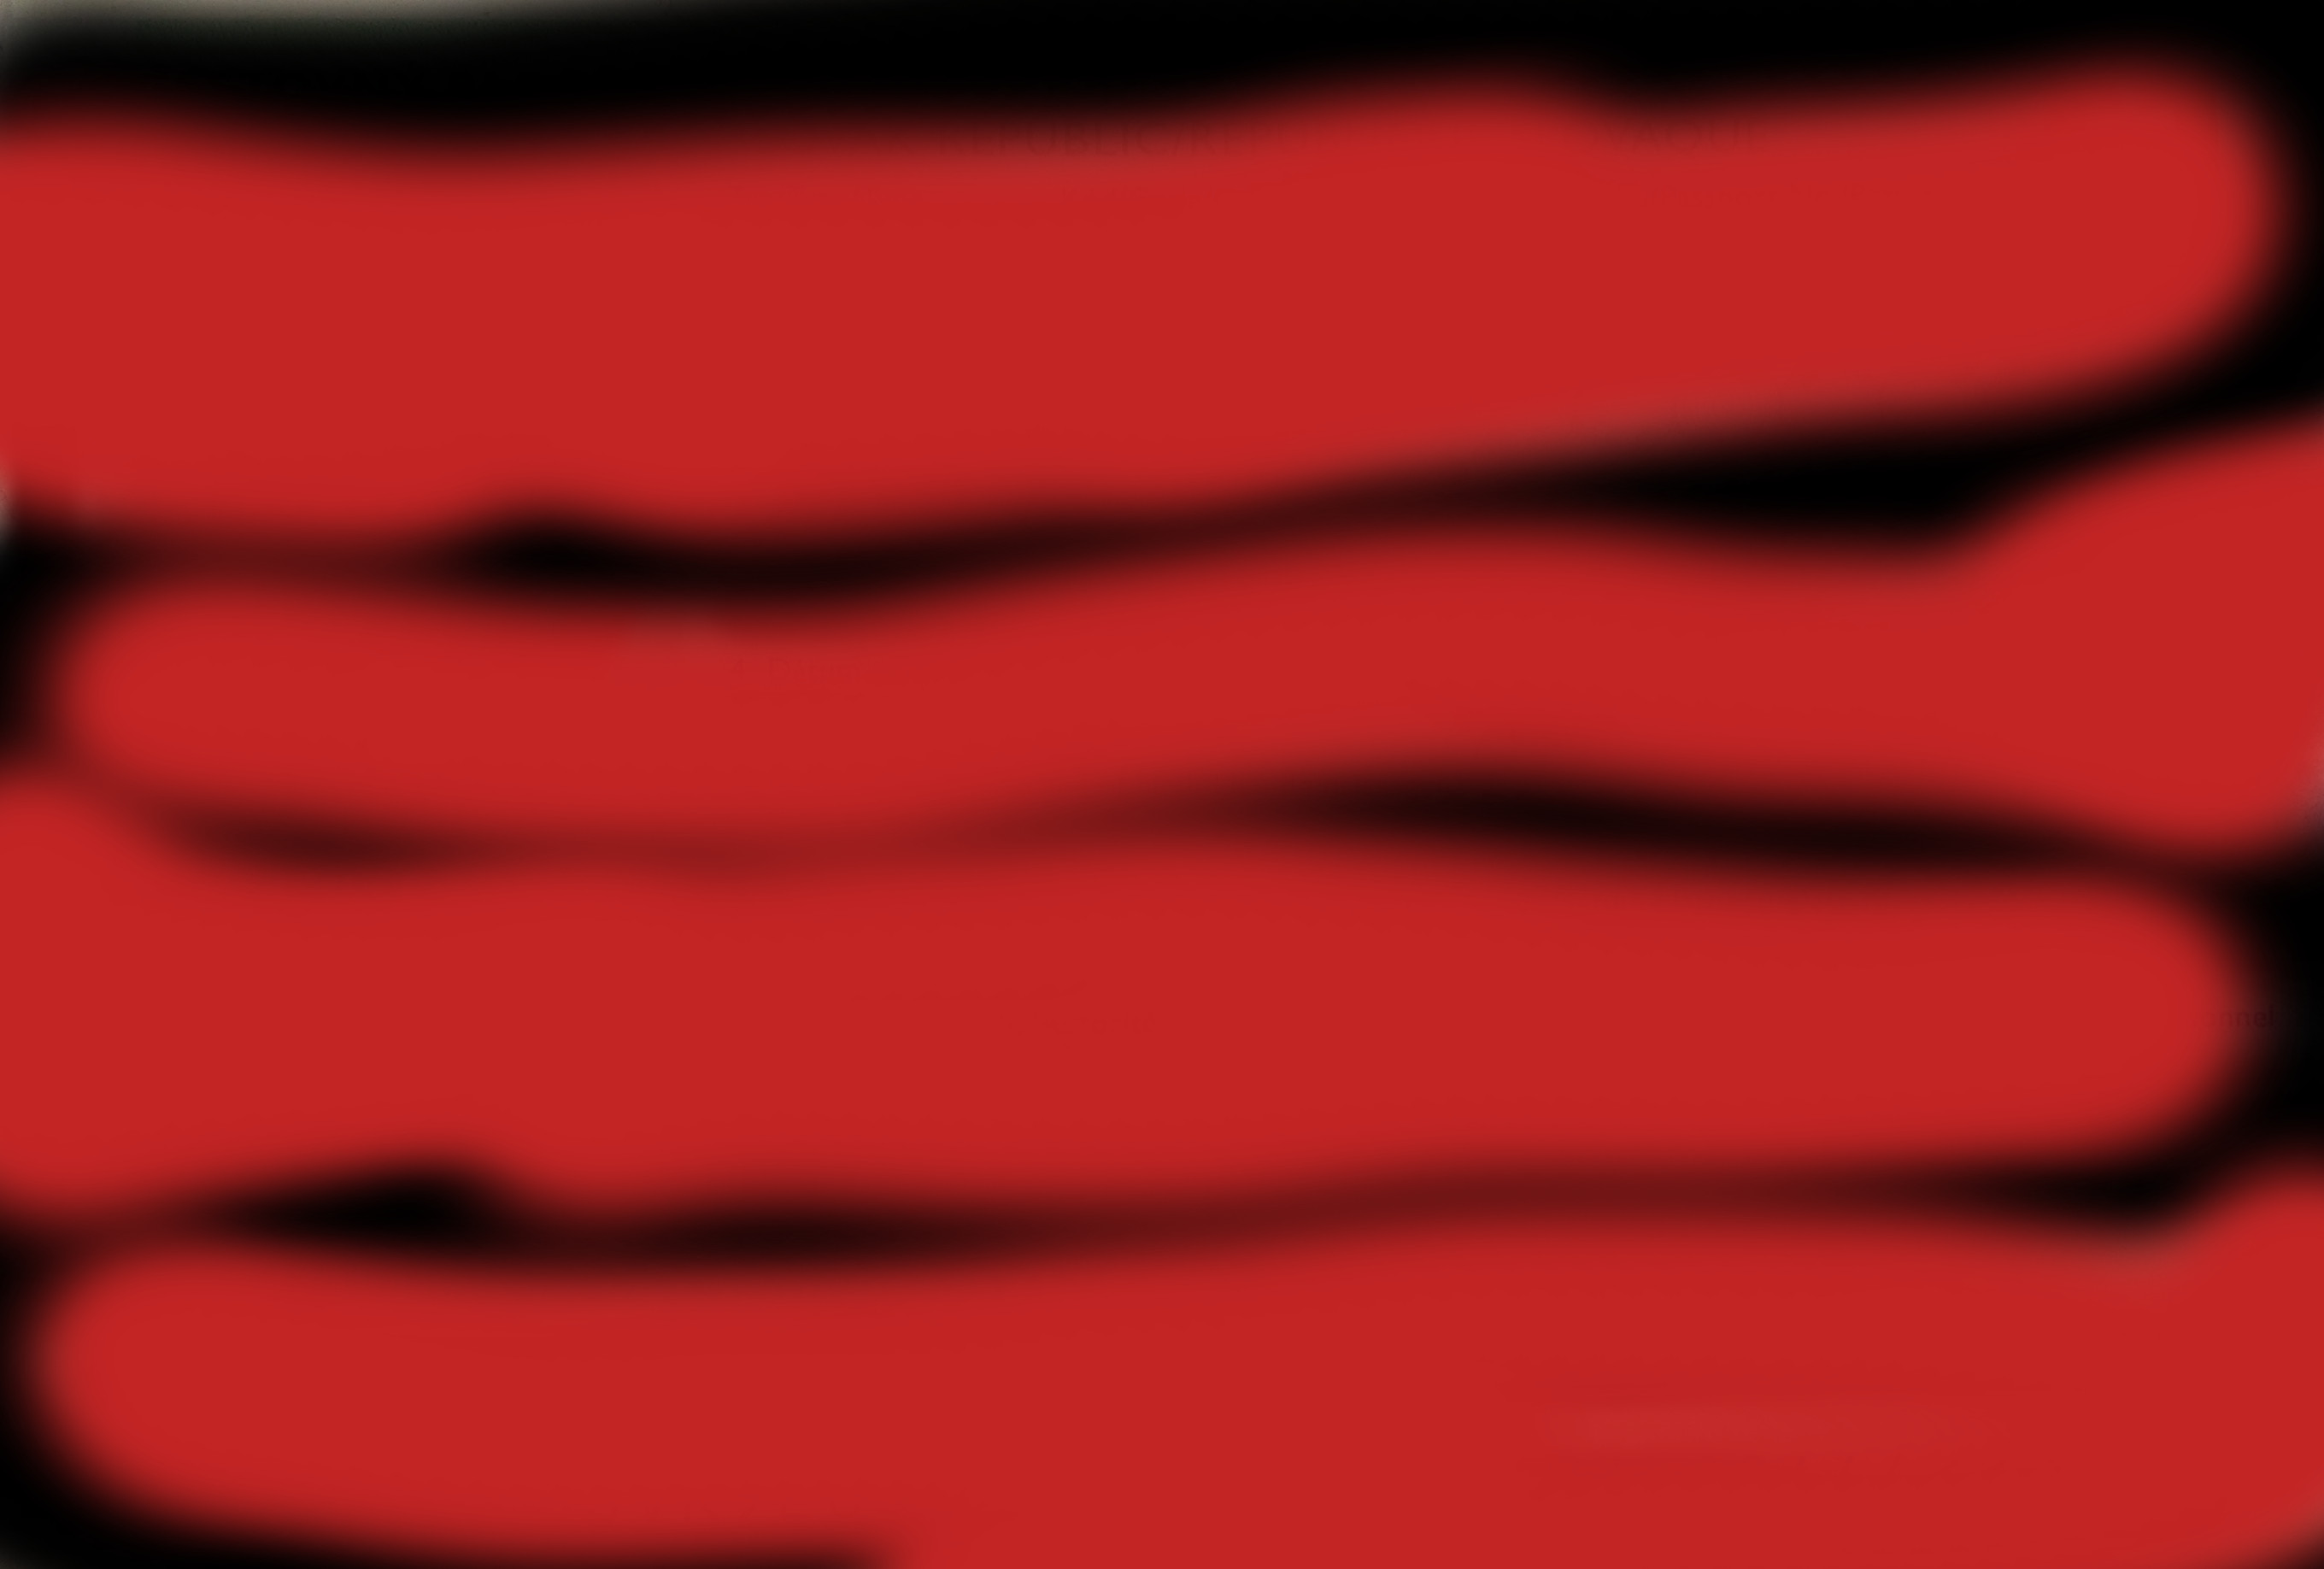
\includegraphics[width=0.8\textwidth]{img/ps.jpg}
\caption{Possible neighborhood functions \cite{Ho03} }
\label{fig:gb}
\end{figure} 	
	
	
\end{introduction}

\setsecnumdepth{all}

%TODO change chapter order and section affiliation.

\chapter{Probability Theory}

This chapter will briefly discuss Discrete-time Hidden Markov Model (later just HMM) as defined in [Rabiner], where you can also look for the more comprehensive explanation with examples.

We have decided to write this chapter, because Continuous-time HMM is its direct logical extension and also it is using some of the subroutines that are the same as if defined for discrete time model.

\section{Discrete Markov Process}\label{sec:DMP}
    
Discrete Markov Process is the stochastic process $X_t$ in discrete equidistant time $\matr{t} = \{ t_1,t_2,\cdots \}$, that in every time occupies some state from the finite state set $\mathcal{S} = \{ s_1, s_2, \cdots, s_n\}$. We will denote as $X_i = s_j$, if the process in time $t$ is in the state $s_j$. The state transition probability will be given in matrix $\matr{A}$, where its elements $a_{ij}, 1\leq i,j \leq n$ represents the probability of the process to move from the state $s_i$ to the $s_j$ in any time step $t$.  Note that $i$ can equal $j$, in that case the process will not move, but it  will remain in the same state. The probability of it is $a_{ii}$.

To tell about the system to be Markov, it should hold so called Markov property. It can be expressed by equation \eqref{eq:mp}. It means that the probability of transition to another state depends only on the current state and doesn't use the information about any past states - the system is memory-less.

\begin{equation}\label{eq:mp}
\begin{aligned}
\mathrm{P}(X_t & = s_j \mid X_{t-1} = s_{j-1}, X_{t-2} = s_{j-2}, \cdots)  \\   
               & = \mathrm{P}(X_t = s_j \mid X_{t-1} = s_{j-1} )
\end{aligned}
\end{equation}

The other important property is Homogeneity. The probability of transition from one state to another is constant throughout the time. 

\begin{equation}\label{eq:homo}
   a_{ij} = \mathrm{P}(X_t = s_j \mid X_{t-1} = s_{j-1} ),\qquad 1 \leq i,j \leq n, \forall t
\end{equation}

For the transition probabilities are applied classical stochastic constrains.

\begin{equation}
   a_{ij} \geq 0
\end{equation}

\begin{equation}
   \sum_{j=1}^n a_{ij} = 1
\end{equation}

\subsection{Discrete-time Hidden Markov Model}

Discrete-time Hidden Markov Model (HMM) is the extension of the previously defined model~\ref{sec:DMP}. In the classic Markov process are the states directly observable. Such a model is often too simplistic to fit well real life problems. The HMM forms the doubly embedded stochastic process, in which the states are not directly observable, but only through the another dependable process, that to every state $s_i$ assign the probability, that it will emit the variable from the set $\mathcal{V}=\{  v_1,v_2,\cdots,v_m\}$. The $\mathcal{V}$ is the set of observable variables. It forms the part of the model, which is known and can be used to guess the possible underlying states chain. The probability of emission of variable $o_j$ by the state $s_i$ will be denoted as $b_i(j)$ and form the matrix $B$, the rectangular matrix of $n$ rows and $m$ columns.
  
To summarize the HMM can be described by its:

\begin{enumerate}[resume]
\setcounter{enumi}{0}
\item \textbf{Hidden States}
\begin{equation}
\mathcal{S} = \{ s_1,s_2, \cdots, s_n \}
\end{equation} 
\item \textbf{State Transition Probability Distribution}
\begin{equation}\label{eq:tp}
\matr{A} = \{ a_{ij} \}, \quad 1 \leq i,j \leq n
\end{equation} 
\item \textbf{Observation Symbols}
\begin{equation}
\mathcal{V} = \{ v_1,v_2, \cdots, v_m \} 
\end{equation}
\item \textbf{Observation Symbols Probability Distribution} \\
$\matr{B} = \{ b_{i}(k) \}$, where $b_{i}(k)$ is the probability that the observation $k$ will occur, if the system is currently in state $i$. 
\begin{equation}
b_i(k) = \mathrm{P}(v_k \text{ at t } \mid X_t = s_i), \qquad 1 \leq i \leq n, \quad 1 \leq k \leq m
\end{equation}
\item \textbf{Initial state distribution} \\
$\pi = \{ \pi_i \}$, where $\pi_i$ is the probability of the initial state being $S_i$.
\begin{equation}
\pi_{i} = \mathrm{P}(X_1 = s_i), \qquad 1 \leq i \leq n
\end{equation}
\end{enumerate}

For the convenience we will declare parameter $\lambda = \{\matr{A},\matr{B},\pi\}$, compactly denoting the set of all parameters of the model. 

\section{Continuous-Time Hidden Markov Model}

All the time we will mention continuous-time hidden Markov model, we will consider its finite states variant. Also the infinite states models exist, but they are out of the scope for these thesis.

In the DT-HMM described in previous chapter, the change of the current state of the process could happen once we moved a step further in the discrete time $t$. The actual state remained hidden, but it has always emitted the observable variable $v_i$.

Comparing to this, in the CT-HMM can change of the state occur at any moment in time (the occurrence holds exponential distribution ). Also it may not be documented by the observation. The emission of the observable variable can happen at any time, however it is independent on the state transition times. For example, it could be times, when the patient undergoes medical examination. The times can generally have highly irregular and unbalanced distribution.

There is much more latent information in such defined model. Not just the hidden states, but also the unknown transition times and unknown state sojourn time (how long will the system remain in the state).
Sometimes the state can change, without emitting a single observation. The large number of hidden information make it to be more complex problem then the discrete time model.

Now we will continue by formally defining Continuous time Markov process, after which we will extend it to the hidden model.

\section{Continuous-Time Markov Process} 

%relationship with discrete (construction)? sum(n = 0..inf) p(n(t)) u(i,j)^n 
%construction from discrete HMM is probably important, heterogenous MM.
%cit:[S.Karlin]
A finite state continuous time Markov process (later as CTMC) is a~stochastic process $X_t (t > 0)$ on the states $\mathcal{S} = \{ s_1, s_2, \cdots, s_n \}$  (for $n>0$ and $\mathcal{S}$ being the finite state set), that in any time $t$  occurs in the corresponding state $1 \leq x_t \leq n$. 

For the times $0 \leq u_0 < u_1 < \cdots < u_r < u$ it satisfies the following equations: 
\begin{itemize}
\item \textbf{Markov property:} Probability of transition from state $i$ to state $j$ during the time interval $t$ is stationary i.e. independent on the states of process in the times $< u$.  
    
\begin{equation}
\begin{aligned}
& \mathrm{P}( x_{t+u} = j \mid x_u = i, x_{u_r} = i_r, \cdots , x_{u_0} = i_0 ) = \\ 
& = \mathrm{P}( x_{t+u} = j \mid x_u = i ), \qquad 1 \leq i,j,i_{0,\cdots,r} \leq n 
\end{aligned}
\end{equation}

The equation describes that the stochastic process is memoryless.

\item \textbf{Homogeneity:} Probability of transition from the state $i$ to $j$ in any given time $s \geq 0$ depends only on the length of the time interval $t \geq 0$. 

\begin{equation}
\begin{aligned}
& \mathrm{P}( x_{t+s} = j \mid x_s = i ) = \mathrm{P}( x_t = j \mid x_0 = i ) = \\
& = \mathrm{p_{ij}}(t)
\end{aligned}
\end{equation}

\end{itemize}
 

The upper mentioned conditions assert, that the transition probability $\mathrm{p_{ij}}(t), 1 \leq i,j \leq S$ satisfies following conditions:%cit:[S.Karlin]


\begin{equation}
\mathrm{p_{ij}}(t) \geq 0
\end{equation}

\begin{equation}
\sum_{j = 1}^n \mathrm{p_{ij}}(t) = 1
\end{equation}

\begin{equation}\label{eq:l0}  
\lim_{t \to 0^+} \mathrm{p_{ij}}(t)= 
\begin{cases}
1, i = j\\
0, i \neq j
\end{cases}
\end{equation}

\begin{equation}\label{eq:ckeq}
\sum_{k = 1}^n\mathrm{p_{ik}}(u)\mathrm{p_{kj}}(t) = \mathrm{p_{ij}}(u+s)     
\end{equation}

Equation \eqref{eq:ckeq} is known as Chapman-Kolmogorov equation. 
We can define the matrix $\mathrm{P_t}$, where the entry $(i,j)$ is $\mathrm{p_{ij}}(t)$ to get the equation in following form:

\begin{equation}\label{eq:ckm}
\matr{P_u} \matr{P_t} = \matr{P_{u+t}},   \qquad t,u > 0  
\end{equation}

?proof of Chapman-kolmogorov?

%construction from Discrete time with poisson timing

\subsection{ Jump Rates }

Using the Chapman-Kolmogorov equation \eqref{eq:ckeq}, if we know the probability $\mathrm{p_{ij}}(t)$ for every states $i,j$ and time $0 < t < t_0$, we are able to compute the values for any time $t > 0$. 
%cit[vytistena st. kniha]

The property \eqref{eq:l0}  asserts that $\mathrm{p_{ij}}(t)$ is continuous for $t=0$. It can be showed from equation \eqref{eq:ckm}, after assigning $t=0$ we will get identity matrix $\matr{P_0} = \matr{I}$.
Moreover from \eqref{eq:ckm} follows that $\mathrm{p_{ij}}(t)$ is continuous for all $t>0$ ref[S.Karlin] and so that there exists the right derivative in 0. This knowledge enables us to determine the $\mathrm{p_{ij}}(t)$ for any given time $t>0$.   

\begin{equation}
q_{ij} =  \left.\frac{\mathrm{d}\mathrm{p_{ij}}(t)}{\mathrm{dt}} \,\right|_{t=0} = \lim_{t \to 0^+} \frac{\mathrm{p_{ij}}(t)}{t}, \quad \text{if } i\neq j     
\end{equation}

We will call this derivative $q_{ij}$ the jump rate from state~$i$ to some other state~$j$. The jump rate $q_{ii}$ can be derived from the equation of transition probabilities summing to the one.

\begin{equation}
1 = \mathrm{p_{ii}}(t) + \sum_{j = 1}^{ n ,j \neq i} \mathrm{p_{ij}}(t) 
\end{equation}

dividing by time interval $t$ and letting $t$ decrease close to zero, we will obtain the following equation. 

\begin{equation}\label{eq:qii}
 q_{ii} =  \sum_{j = 1}^{ n ,j \neq i} q_{ij} 
\end{equation}

(We assume the finite rates $q_{ij}$, infinite rate would immediately lead to the leaving of the state, so it makes no sense for us to consider.)

It can be shown that by construction of the CTMC from discrete time Markov chain (DTMC) and  it's underlying Poisson process with rate $\lambda$, the equation $q_{ij} = \lambda a_{ij}$ holds. Where $a_{ij}$ is the transition probability from the $i$ to $j$ in DTMC \ref{eq:tp}. This is why we call the $q_{ij}$ the jump rate.[zdroj]  

%ROUTING MATRIX - u(i, j) = q(i, j) / lambda max
%u(i, i) = 1 - sum_j u(i, j)

We can also look at $q_{ii}$ as at the rate in which the $X_t$ is leaving the state $i$ \eqref{eq:ckeq}. Then we can define the jump rates matrix $\matr{Q}$ as following:

\begin{equation}
\begin{aligned}  
\matr{Q}(i,j)= 
\begin{cases}
\qquad q_{ij}, \qquad & \text{if } i\neq j\\
\sum\limits_{k = 1}^{ n ,k \neq i} q_{ik}, \qquad & \text{if } i=j
\end{cases}
\end{aligned}
\end{equation}

Such a defined matrix will hold $\pi\matr{Q} = 0$... [explain more, proof, $e^{\matr{Q}t}$]

\subsection{Construction from Discrete-Time Markov Process with Poisson Process Timing } 

The useful way to the understanding of the continuous-time Markov process is by its relation to the discrete process, that can be shown by the construction.

We will take the homogeneous Poisson process $N(t)$ with parameter $\lambda$ and the discrete-time Markov process $Y_n$, with the transition probabilities $a_{ij}$. With the $N(t)$ and $Y_n$ being mutually independent. To make the construction, we will change the equidistant timing of $Y_n$ by Poisson process timing. We will get the process $Y_{N(t)}$ in which the transition from the state $i$ happens at each arrival in $N(t)$ with the probability $a_i = \sum_{j = 1}^{ n ,j \neq i} a_{ij}$ (notice that the transition will not occur if $i=j$) and the sojourn time in state $i$ will be exponentially distributed with the parameter $q_i$, what is $\mathrm{f}(t)= a_i e^{-a_i t}$. Such a process $X_t = Y_{N(t)}$ is called continuous-time Markov process.

Now we can derive the equation for probability of transition from the state $i$ to the state $j$ in the time $t$ as the sum of all the possible number of steps in which the transition can occur. 

\begin{equation}
\begin{aligned}
\mathrm{p_t(i,j)} &= \sum_{n=0}^{\infty} \mathrm{P}( N(t) = n, Y_t = s_j \mid Y_t = s_i )  = \\
                  &= \sum_{n=0}^{\infty} \mathrm{P}( N(t) = n, Y_{N(t)} = s_j \mid Y_{N(t)} = s_i )  = \\
                  &= \sum_{n=0}^{\infty} \mathrm{P}( N(t) = n ) \mathrm{P}( Y_n = j \mid Y_0 = i )  = \\
				  &= \sum_{n=0}^{\infty} e^{-\lambda t} \frac{ (\lambda t)^n}{n!} a_{ij}^n  
\end{aligned}
\end{equation} 


%ref Yu-Ying Liu

\subsection{ Fully Observable Continuous-Time Markov Process }

Let's have continuous time Markov chain on the state space $\mathcal{S}$, with the jump rates in the matrix $\matr{Q}$, initial state probability distribution $\pi$ and the known transitions to the corresponding states $\matr{X^{'}}= ( x_0, x_1, \cdots, x_{v^{'}} ) $ occurring at times $\matr{T^{'}} = ( t_0^{'}, t_1^{'}, \cdots, t_{v^{'}}^{'} )$. Such a system, where we know, when and where the transition will happen is called fully observable and we can count its complete likelihood ($\mathcal{L}_{FO}$). 

\begin{equation}\label{eq:CL1}
\begin{aligned}  
 \mathcal{L}_{FO} &=  \prod_{u=0}^{v^{'}-1} ( q_{x_u x_{u+1}} / q_{x_u} )( q_{x_u} e^{ - q_{x_u} \tau_{u }^{'}}) = \\
    &= \prod_{u=0}^{v^{'}-1} q_{x_u x_{u+1}} e^{ - q_{x_u} \tau_{u}^{'}}
\end{aligned}
\end{equation}

where the $q_i = \sum_{j=1}^{n,i\neq j} q_{ij}$ is the probability of transition from the state~$i$ and   
$\tau_{u}^{'} = t_{u+1}^{'} - t_{u}^{'}$ is the time interval among the two consecutive steps.

The equation can be further rearranged in the form that group together the same state transition. The variable $\eta_{ij}$ marks the number of transition $q_{ij}$ that have occurred and the~$\tau_i$ is the total time spend in the state~$s_i$.

\begin{equation}\label{eq:CL2}
 \mathcal{L}_{FO} = \prod_{i=1}^{n} \prod_{j=1}^{n, i \neq j} q_{ij}^{\eta_{ij} } e^{ - q_i \tau_i }
\end{equation}

\subsection{ General Continuous-Time Markov Process }

In general we do not know the state of the system during all the time. It is only known at some unevenly distributed times $\matr{T} = ( t_0, t_1, \cdots, t_{v} )$ as $\matr{X}= (x_0, x_1, \cdots, x_{v} )$. 
This add an amount of insecurity in the probability computation. We do not longer know, the number of transitions $\eta_{ij}$ as well as the time spend in the specific state $\tau_i$. 

To count the likelihood of the chain, we will use earlier defined matrix $\matr{P}(t)$ and its elements $\mathrm{p_{ij}}(t)$ [ref] for the time interval~$\tau_u = t_{u+1} - t_u$.    

\begin{equation}
 \mathcal{L} = \prod_{u=0}^{v-1} \mathrm{p}_{x_u x_{u+1}}(\tau_u) 
\end{equation}

It can be alternatively extended in the form

\begin{equation}
 \mathcal{L} = \prod_{u=0}^{v-1} \prod_{i=0,j=0}^{n}  \mathrm{p}_{ij}(\tau_u)^{\mathbb{I}( x_u = i, x_{u+1} = j )} 
\end{equation}

where the function $\mathbb{I}(i,j)$ equal either $1$, if both condition inside are true, or $0$ if they are not. 
If the variable $r$ - the number of all distinct time intervals $\tau_{\Delta}, \Delta =\{1,2,\cdots,r\}$ is lower then number of observations, it could be beneficial to aggregate them as in formula,

\begin{equation}\label{eq:CTL}
 \mathcal{L} = \prod_{\Delta = 1}^{r} \prod_{i=0,j=0}^{n}  \mathrm{p}_{ij}(\tau_{\Delta})^{\mathbb{C}( \tau=\tau_{\Delta} x_u = i, x_{u+1} = j )} 
\end{equation}

where function $\mathbb{C}$ denotes the total number of intervals, for that condition is true.
    
%TODO P_{ij}(t) counting possibilities.

\section{Continuous-Time Hidden Markov Model}

Continuous-time hidden Markov model is the extension of CTMC, where the states in times $\matr{T} = ( t_0, t_1, \cdots, t_{v} )$ are not directly observed, just seen as the observation symbols sequence $\matr{O} = \{  o_0, o_1, \cdots, o_{v} \}$, emitted by the current state $s_i$ with the probability $b_i(o)$.
The likelihood of the completely observed system  $\mathcal{L}_{FO}$ will be similar to the $\mathcal{L}_{FO}$ of CTMC \eqref{eq:CL1} \eqref{eq:CL2} with the difference we need to take into account the probability of actual observation.

\begin{equation}\label{eq:HMCL1}
\begin{aligned}  
 \mathcal{L}_{FO} &= \prod_{u^{'}}^{u^{'}-1} q_{x_{u^{'}} x_{u^{'}+1}} e^{ - q_{x_{u^{'}}} \tau_{u^{'}} } 
    \prod_{u=0}^v b_{ x_u }(o_u) = \\
    &= \prod_{i=1}^{n} \prod_{j=1}^{n, i \neq j} q_{ij}^{\eta_{ij} } e^{ - q_i \tau_i } \prod_{u=0}^v b_{x_u}(o_u)
\end{aligned}
\end{equation}
%TODO s(t_v) was not defined enywhere, it need to be unified with the notation q_t = S from discrete model!

%TODO Move the CT-HMM intorduction in here, and separate it in the more chapters, not the EM- chapter. 
 

\chapter{Statistic Theory}


\section{Expectation-Maximization Algorithm}\label{ch:EM}


%(1) Maximum Likelihood from Incomplete Data via the EM Algorithm , A. P. Dempster; N. M. Laird; D. B. Rubin, Journal of the Royal Statistical Society. Series B (Methodological), Vol. 39, No. 1. (1977), pp.  1-38.

Expectation-Maximization (EM) Algorithm (first introduces in [1]) is the method for finding the Maximum likelihood estimates(MLE) of parameters in probabilistic models over the incomplete data-set ( i.e. data-set containing unobserved (latent) variables ). It is a natural generalization of maximum likeli-
hood estimation, however the latent variables makes finding of the MLE more difficult. To count it directly can be very computationally expensive, so the EM algorithm use the iterative approach to approximate the solution by repeating the sequence of simpler consecutive steps.

Let's have vector $\mathbf{x} = (x_{1},x_{2},\dotsc,x_{n})$ containing the known (observed) variables and vector $\mathbf{z} = (z_{1},z_{2},\dotsc,z_{n})$ containing latent (unobserved) variables. We will set $\theta$ for the unknown parameters we want to estimate. We will use the notation $\mathrm{logP}(\mathbf{x},\mathbf{z};\theta)$ as the log-likelihood function, which estimates the probabilities for the given parameters. Notice that we are using the log-likelihood to avoid underflow of parameters values that could otherwise easily arise during the computation.  
%[st]simle tutorial: What is the expectation maximization algorithm? Chuong B Do & Serafim Batzoglou

Look at [st] for more detailed, easily understandable tutorial with examples.    

\begin{enumerate}
\item \textbf{Initialization:} We will make the initial guess of the parameters $\hat \theta^{(0)} $.
\end{enumerate} 

We will continue by iterating through two following steps: 

\begin{enumerate}[resume]
\item \textbf{Expectation:} Calculate the expected value of the likelihood function $\mathrm{logP}(\mathbf{x},\mathbf{z};\hat \theta^{(t)})$. Where $\hat \theta^{(0)}$ is the current parameters estimation. We will find the function $\mathrm{Q}$ that lower bounds $\mathrm{logP}(\mathbf{x},\mathbf{z};\hat \theta^{(t)})$.

\begin{equation}\label{eq:exp}
 \mathrm{Q}(\hat\theta^{(t)}) =  \mathrm{logP}(\mathbf{x},\mathbf{z};\hat \theta^{(t)})
\end{equation}

\item \textbf{Maximization:} Find the value $\hat\theta^{(t+1)}$ that maximize $\mathrm{Q}(\hat\theta^{(t)})$.  
\end{enumerate}  

As the value of $\mathrm{Q}(\hat\theta^{(t)})$ matches the log-likelihood function at $\hat\theta^{(t)}$, it follows that $ \mathrm{Q}(\hat\theta^{(t)}) =  \mathrm{logP}(\mathbf{x},\mathbf{z};\hat \theta^{(t)}) \leq \mathrm{Q}(\hat\theta^{(t+1)}) =  \mathrm{logP}(\mathbf{x},\mathbf{z};\hat \theta^{(t+1)}) $ thus the function value form the non-decreasing order. [nejaky dokaz?]. We will stop the computation ones the parameter converges to some value, that is not changing.  

It is important to notice that this approach leads to the local optimum. To get better results the algorithm can be launched more times starting always with different random initialization. So much some other optimization technique can be used [sources?]. 

\section{Three Basic Problems for HMMs}\label{sec:3p}
% citate: Jack Ferguson of IDA in lectures at Bell laboratories
When dealing with real-world application we need to deal with following problems, as proposed in [citace]. First we will describe the problems and later in the successive subsections we will explain the algorithms that can effectively solve them. 

\begin{enumerate}
\item Compute the probability $\mathrm{P}(\matr{O}|\lambda) $ of the observation sequence \\ $\matr{O} = (o_1,o_2,\cdots,o_T)$, given the set of parameters $\lambda = \{A,B,\pi\}$. Elements of the observation sequence $\matr{O}$ are some specific measured data, taking values from the set~$\mathcal{V}$.   
\item Choose the optimal state sequence $\matr{X} = (x_1,x_2,\cdots,x_T$), having the observation sequence $\matr{O}$ and parameters $\lambda$.
\item Adjust the model parameters $\lambda$ in the way it maximizes the probability of observation sequence $ \mathrm{P}(\matr{O}|\lambda) $. 
\end{enumerate}


\subsection{Forward-Backward Algorithm}\label{sec:fb}
The Forward-Backward Algorithm is actually the pair of two separate algorithms (Forward vs. Backward). We will explain the Forward one and at the end we will describe the modifications that are needed to do the Backward. Both of them are sufficient for solving of the first proposed problem, however we need to define both of them for the later use in the text.  

Forward Algorithm is the Dynamic Programming algorithm building upon the Markov property - the independence upon past events. We will denote the forward variable as $\alpha_t(i)$ defined as the probability of partial observation sequence, with the last observation in time $t$ emitted by the state $s_i$, all given the parameters $\lambda$.

\begin{equation}
\alpha_t(i) = \mathrm{P}(o_1,o_2,\cdots,o_t,X_t = s_i \mid \lambda )
\end{equation}

that can be gradually counted by following equations for $t=1$ and $t=t+1$ using bottom-up strategy.

\begin{equation}
\alpha_1(i) = \pi_i b_i(o_1), \qquad 1 \leq i \leq n
\end{equation}

\begin{equation}
\begin{aligned}
\alpha_{t+1}(i) = \left( \sum_{j=1}^n \alpha_t(j) a_{ji} \right) b_i(o_{t+1}), \qquad 1& \leq t \leq T - 1, \\ 
                                                                                 1& \leq i \leq n		\end{aligned}
\end{equation}

Now we can obtain the solution of the first problem simply by summing through the all forward variables in the time $T$.

\begin{equation}
\mathrm{P}(\matr{O}|\lambda) = \sum_{i=1}^n \alpha_T(i)
\end{equation} 

Similarly we can define backward variable $\beta_t(i)$ as
\begin{equation}
\beta_t(i) = \mathrm{P}(o_{t+1},o_{t+2},\cdots,o_T,X_t = s_i \mid \lambda ) 
\end{equation}
The DP algorithm can be derived analogically as the one for the Forward procedure, with the single difference, that it will start counting from the end, so the total probability can be count by summing the backward variables in time $t=1$.

We need to count $n$ variables at each time-step, each of that takes exactly $n$ steps to evaluate. It makes overall complexity $\mathcal{O}(n^2T)$.    

\subsection{Individually Most Likely States Sequence}\label{sec:ssp}
There is more ways how we can look at the world "optimal" in the problem 2 statement. One of the possible approaches is to maximize the expected number of correctly assigned states. To solve it, we need to define the variable determining the probability of being in specific state in particular time.

\begin{equation}
\gamma_t(i) = \mathrm{P}(X_t = s_i \mid \matr{O},\lambda ) 
\end{equation}

Here we can use already defined forward and backward variables and count the $\gamma_t(i)$ as
\begin{equation}
\begin{aligned}
\gamma_t(i) &= \frac{ \mathrm{P}( X_t = s_i, \matr{O} \mid \lambda )}{ \mathrm{P}( \matr{O} \mid \lambda )} =
               \frac{  \alpha_t(i) \beta_t(i) }{ \mathrm{P}( \matr{O} \mid \lambda )} = \\
            &= \frac{  \alpha_t(i) \beta_t(i) }{ \sum\limits_{j=1}^n \alpha_t(j) \beta_t(j) } 
\end{aligned}
\end{equation}

To get the desired individual most likely state $x_t$, it is enough to find one of the highest probability.

\begin{equation}
x_t = \argmax_{1 \leq i \leq n} \gamma_t(i), \qquad 1 \leq t \leq T
\end{equation} 

Applying this algorithm to the whole sequence will lead to the highest expected number of correctly assigned states, however such a sequence as a whole can have low probability or in some extreme cases can not even be feasible. This would happen if probability of transition among two consecutive states in the sequence was zero.   
   
\subsection{Viterbi Algorithm} 

An another way how to look on the problem 2 is to find single most probable state sequence. It means to maximize $\mathrm{P}(\matr{X}\mid \matr{O},\lambda)$, what is equivalent to maximize $\mathrm{P}(\matr{X}, \matr{O}\mid\lambda)$. %TODO is \matr{X} defined?

Viterbi Algorithm is the Dynamic Programming algorithm, that similarly to the Forward-Backward algorithm  benefits from memorylessness of Markov Chain. In DP we can gradually count the variable $\delta_t(i)$, that represents the maximal probability of the state chain from $time = 1$ till $t-1$, with the current state being $s_i$.

\begin{equation}\label{eq:delta}
\delta_t(i) = \max_{x_1,x_2,\cdots,x_{t-1}} \mathrm{P}( x_1,x_2,\cdots, x_t = s_i, o_1, o_2, \cdots, o_t \mid \lambda )
\end{equation} %TODO x_t = s_i, or X_t = s_i

To get the actual state sequence, we need to store the information about the state that has maximized in the previous equation \eqref{eq:delta}. We will store it in the array $\psi_t(i)$. Now we can define the initialization of the algorithm as

\begin{equation}
\delta_1(i) = \pi_i b_i(o_1), \qquad 1 \leq i \leq n 
\end{equation}

\begin{equation}
\psi_1(i) = 0 
\end{equation}

and consecutive bottom-up computation as

\begin{equation}
\begin{aligned}
\delta_{t}(i) = ( \max_{ 1 \leq j \leq n } \delta_{t-1}(j)a_{ji} ) b_i(o_{t}), \qquad 2& \leq t \leq T, \\
																					   1& \leq i \leq n
\end{aligned}
\end{equation}

\begin{equation}
\begin{aligned}
\psi_{t}(i) = ( \argmax_{ 1 \leq j \leq n } \delta_{t-1}(j)a_{ji} ), \qquad \qquad 2& \leq t \leq T, \\
																			       1& \leq i \leq n
\end{aligned}
\end{equation}

Now we can get the searched state sequence probability 

\begin{equation}
\mathrm{P}^* = \max_{1 \leq i \leq n} ( \delta_{t}(i) )  
\end{equation}

and the actual state path by backtracking

\begin{equation}
x_t^* = \argmax_{1 \leq i \leq n} ( \delta_{t}(i) ),  \qquad t = T  
\end{equation}

\begin{equation}
x_t^* = \psi_{t+1}(x_{t+1}^*), \qquad t = T-1, T-2, \cdots, 1  
\end{equation}

The structure of the algorithm is very similar to the Forward-Backward algorithm, so we can easily see its complexity is also $\mathcal{O}(n^2T)$.

\subsection{Baum-Welch Algorithm}\label{sec:BWA}

There doesn't exist analytic solution for the problem~3. There are more possible iterative algorithms from which we will describe the expectation-maximization approach~\ref{ch:EM}, based on the classic work of Baum and his colleagues.[ref?] We will start by defining the variable~$\xi_t(i,j)$ as the probability~of being in the state~$s_i$ in the time~$t$ and in state~$s_j$ in the time~$t+1$. 

\begin{equation}
\xi_t(i,j) = \mathrm{P}( X_t = s_i, X_{t+1} = s_j \mid \matr{O}, \lambda )  
\end{equation}

The probability can be compute using forward-backward variables as follows
 
\begin{equation}\label{eq:xi}
\begin{aligned}
\xi_t(i,j) &= \frac{ \alpha_t(i) a_{ij} b_j(o_{t+1}) \beta_{t+1}(j) }
		   		   { \mathrm{P}( \matr{O} \mid \lambda ) } \\
		   &= \frac{ \alpha_t(i) a_{ij} b_j(o_{t+1}) \beta_{t+1}(j) }
		   		   { \sum\limits_{i=1}^n \sum\limits_{j=1}^n \alpha_t(i) a_{ij} b_j(o_{t+1}) \beta_{t+1}(j) }
\end{aligned}
\end{equation}

Obviously it is in relation with already defined variable~$\gamma_t(i)$ - the probability of being in the state~$s_i$ in the time~$t$.

\begin{equation}
\gamma_t(i) = \sum_{j=1}^n \xi_t(i,j)  
\end{equation}

We can get the expected number of transitions from~$s_i$, when summing~$\gamma_t(i)$ over the time till~$T-1$. Similarly we would get expected number of times in~$s_i$, by summing over~$t$ from~$t=1$ till~$t=T$. 

\begin{equation}
\mathbf{E}(\text{transitions from $s_i$}) = \sum_{t=1}^{T-1} \gamma_t(i)  
\end{equation}

If summing~$\xi_t(i,j)$ over the time, we will get expected number of transitions from $s_i$ to $s_j$, . 

\begin{equation}
\mathbf{E}(\text{transitions from $s_i$ to $s_j$}) = \sum_{t=1}^{T-1} \xi_t(i,j)  
\end{equation}

Now we have all what is needed to define the reestimated model~$\hat\lambda=(\hat{\matr{A}},\hat{\matr{B}},\hat\pi)$.

\begin{equation}\label{eq:bwpi}
\hat\pi_i = \gamma_1(i)  
\end{equation}

\begin{equation}\label{eq:bwa}
\begin{aligned}
\hat a_{ij} &= \frac{\mathbf{E}(\text{transitions from $s_i$ to $s_j$})}
				   {\mathbf{E}(\text{transitions from $s_i$})}  \\
		    &= \frac{\sum\limits_{t=1}^{T-1} \xi_t(i,j)}{\sum\limits_{t=1}^{T-1} \gamma_t(i) }
\end{aligned}
\end{equation}

\begin{equation}\label{eq:bwb}
\begin{aligned}
\hat b_{i}(k) &= \frac{\mathbf{E}(\text{times of visiting $s_i$ and observing symbol $v_k$ })}
				   {\mathbf{E}(\text{times of visiting $s_i$})} \\
			  &= \frac{\sum\limits_{t=1, \text{if } O_t = v_k  }^{T} \gamma_t(i)}{\sum\limits_{t=1}^{T} \gamma_t(i) } 
\end{aligned}
\end{equation}

%TODO O_t = v_k, ok?

The formulas can be interpreted as the steps of EM-algorithm, with the expectation step being the computation of auxiliary function~$Q(\lambda,\hat\lambda)$ and maximization step, the maximization over parameter~$\hat\lambda$. The algorithm will stop ones it is no longer improving (re-estimation doesn't bring higher probability). It is important to notice, that the found solution is the local optimum, the searched space can be very complicated containing many local optima, that's way it can helpful to start the algorithm more times with different parameter initialization.  

%proof it is growing { was mentioned in EM }

\subsection{EM Algorithm} 

There is no available analytic maximizer of likelihood function \eqref{eq:CTL}, however it can be estimated iteratively by the EM algorithm proposed in [ref:PhysRevE.76].  
For the expectation step we will use logarithms of expected complete likelihood function \eqref{eq:CL2}, with the estimated parameter of $\matr{Q}$ in step $t$ noted as $\matr{ \hat Q_t } $.

\begin{equation}\label{eq:EMCL}
 \ln( \mathcal{L}_{FO} ) = \sum_{i=0}^n \sum_{j=0}^{n, i \neq j} \ln( \hat q_{ij}) \mathbf{E}( \eta_{ij} \mid \matr{X}, \matr{ \hat Q_t } ) - \hat q_i \mathbf{E}( \tau_i \mid \matr{X}, \matr{ \hat Q_t } )
\end{equation}

In the maximization step we will evaluate new values for $\matr{ \hat Q }$, so that the previous equation was maximized. 

\begin{equation}
\begin{aligned}  
\matr{ \hat Q_t }(i,j)= 
\begin{cases}
\frac{ \mathbf{E}(\eta_{ij} \mid \matr{X}, \matr{ \hat Q_t } )}{ \mathbf{E}( \tau_i \mid \matr{X}, \matr{\hat Q_t} ) } & \text{if } i\neq j\\
- \sum\limits_{k=1}^{n,k \neq i} q_{ik}, \qquad & \text{if } i=j
\end{cases}
\end{aligned}
\end{equation}

Now, there remain the non-trivial task to evaluate $\mathbf{E}( \eta_{ij} \mid \matr{X}, \matr{\hat Q_t} )$ and $\mathbf{E}( \tau_i \mid \matr{X}, \matr{ \hat Q_t } )$. They can be expressed as following sums.


\begin{equation}
\begin{aligned}  
\mathbf{E}(\eta_{ij} \mid \matr{X}, \matr{\hat Q_t} ) &= \sum_{u=0}^{v-1} \mathbf{E}(\eta_{ij} \mid x_u, x_{u+1}, \matr{ \hat Q_t } ) = \\
&= \sum_{u=0}^{v-1} \sum_{k=0,l=0}^{n} \mathbb{I}( x_u = k, x_{u+1} = l ) \mathbf{E}(\eta_{ij} \mid x_u = k, x_{u+1} = l, \matr{\hat Q_t} )
\end{aligned}
\end{equation}


\begin{equation}
\begin{aligned}  
\mathbf{E}( \tau_i \mid \matr{X}, \matr{\hat Q_t} ) &= \sum_{u=0}^{v-1} \mathbf{E}(\tau_i \mid x_u, x_{u+1}, \matr{ \hat Q_t } ) = \\
&= \sum_{u=0}^{v-1} \sum_{k=0,l=0}^{n} \mathbb{I}( x_u = k, x_{u+1} = l ) \mathbf{E}(\tau_i \mid x_u = k, x_{u+1} = l, \matr{\hat Q_t} )
\end{aligned}
\end{equation}
   
With the use of the Markov property and from homogeneity of the Markov process, the computations may be reduced to computing of expected values, for all foursome of $i,j,k,l \in S$. It will be showed later in the text[future ref].     
   
\section{The Model Parameters Estimation}
%viterbi forward-backward need to be redefined with different rates matrix for different interval.

%continuous time Baum-Welch -> citace veci, ktore to robili - DP, spaniely, starsi clanok. + preco je novsi clanok najlepsi.

For the model parameters estimation in DT-HMM, we have used the already long known Baum-Welch algorithm \ref{sec:BWA}. We can use the same approach for the estimation of parameters $\hat \pi$ \eqref{eq:bwpi} and $\matr{ \hat B }$ \eqref{eq:bwb}. Just we need to use the time dependent jump rates instead of time-homogeneous transition probabilities. %TODO define new \gamma \chi ? maybe will be done in Posterior.  

However the estimation of the $\matr{ \hat Q }$ can't be inherited from the discrete model, because the state transitions are not dependent on the observation times and there can even be more of them between two observations. The following algorithm proposed in the article [ref:YuYingLiu], was the first which could efficiently solve the issue.        

The expectation step will be the log-likelihood of the model. Simply just the logarithm of the full observation probability function \eqref{eq:HMCL1}.

\begin{equation}\label{eq:EMCTHMM}
\begin{aligned}  
 \ln(\mathcal{L}_{FO}) &= \sum_{i=1}^{n} \sum_{j=1}^{n, i \neq j} \big( \ln( \hat q_{ij}) \mathbf{E}( \eta_{ij} \mid \matr{O},\matr{T}, \matr{ \hat Q_t } ) - \hat q_i \mathbf{E}( \tau_i \mid \matr{O},\matr{T}, \matr{ \hat Q_t } ) \big) + \\
    &+ \sum_{u=0}^v \mathbf{E}( \ln( b_{ x_u }(o_u) ) \mid, \matr{O},\matr{T},\matr{\hat Q_t} )
\end{aligned}
\end{equation}

We will maximize the previous function by recalculating the~$\matr{ \hat Q_t }$. 

\begin{equation}\label{eq:Qmax}
\begin{aligned}  
\matr{ \hat Q_t }(i,j)= 
\begin{cases}
\frac{ \mathbf{E}(\eta_{ij} \mid \matr{O},\matr{T}, \matr{ \hat Q_t } )}{ \mathbf{E}( \tau_i \mid \matr{O},\matr{T}, \matr{\hat Q_t} ) } & \text{if } i\neq j\\
- \sum\limits_{k=1}^{n,k \neq i} q_{ik}, \qquad & \text{if } i=j
\end{cases}
\end{aligned}
\end{equation}


The challenging step is to derive computation of expected values of $\eta_{ij}$ and $\tau_i$. We will start with the first $\mathbf{E}(\eta_{ij} \mid O,T, \hat Q_t )$, which will be expressed as the sum through all possible state sequences.

\begin{equation} 
\sum_{x_1,\cdots,x_v)} p(x_1,\cdots,x_v) \mid \matr{O},\matr{T}, \matr{ \hat Q_t }) \mathbf{E}(\eta_{ij} \mid x_1,\cdots,x_v) ,\hat Q_t )
\end{equation}

The expectation part can be rewrite in the intervals form.  

\begin{equation}
 \sum_{x_1,\cdots,x_v)} p(x_1,\cdots,x_v \mid \matr{O},\matr{T}, \matr{ \hat Q_t }) \sum_{u=1}^{v-1}\mathbf{E}(\eta_{ij} \mid x_u, x_{u+1} ,\matr{\hat Q_t} )
\end{equation}

Because the Markov condition hold, we can interval-wise divide the complex probability function and for every of the time intervals sum through all possible states $k,l$ at its edge. 

\begin{equation}
\sum_{u=0}^{v-1} \sum_{k=0,l=0}^n p( x_u = k, x_{u+1} = l \mid \matr{O},\matr{T}, \matr{ \hat Q_t }) \mathbf{E}(\eta_{ij} \mid x_u = k, x_{u+1} = l, \matr{ \hat Q_t } )
\end{equation}

The expected value of sojourn time $\mathbf{E}( \tau_i \mid \matr{O},\matr{T}, \matr{ \hat Q_t } )$ can be derived equivalently.

\begin{equation}
\sum_{u=0}^{v-1} \sum_{k=0,l=0}^n p( x_u = k, x_{u+1} = l \mid \matr{O},\matr{T}, \matr{ \hat Q_t }) \mathbf{E}(\tau_i \mid x_u = k, x_{u+1} = l,\matr{\hat Q_t} )
\end{equation}

In the following section \ref{sec:pos}, we will show, how to count $p(x_u = k,x_{u+1} = l \mid \matr{O},\matr{T}, \matr{ \hat Q_t })$. The remaining part of computing $\mathbf{E}(\eta_{ij} \mid x_u = k, x_{u+1} = l,\matr{\hat Q_t} )$ and $\mathbf{E}(\tau_i \mid x_u = k, x_{u+1}) = l, \matr{ \hat Q_t } )$ will be presented in \ref{sec:endexp}. 

\section{The Posterior State Probabilities}\label{sec:pos}

We have introduced the tree basic problems of DT-HMM in section \ref{sec:3p}. They can be likewise defined for the continuous model. We have already shown the partial solution of the third problem (model parameters adjustment) in the previous section, now we will discuss the first two problems. We will show that to solve them, we need only little transformation of DT-HMM algorithms.

To count the probability of the CT-HMM with specified parameters, and defined states in observation points, we do not need to know about the state transition that have occurred among the observations.
If we take this observation into the account, we can look on the model as it was the time in-homogeneous DT-HMM. It is the model, in which the state transition probabilities can change in every time-step. We have previously defined the transition probability from state $i$ to the state $j$ in time interval $\tau$ as $p_{i,j}( \tau ) = e^{ \matr{Q} \tau}$, that can play the role of the transition probabilities in discrete time in-homogeneous model. Now we can define the desired probability as following:

\begin{equation}
\prod_{u=1}^{v-1} p_{x_u, x_{u+1}}(\tau_u) \prod_{u=1}^{v} b_{ x_u }(o_u)
\end{equation}

It should be obvious now, that for the continuous variant of Viterbi and Forward-backward algorithm, we only need to change the state transition $a_{ij}$ to time variable~$p_{i,j}( \tau_u )$.   
Now, we have everything what we need for counting the posterior state distribution $p( x_u = k, x_{u+1} = l \mid \matr{O},\matr{T}, \matr{ \hat Q_t } )$, using the forward and backward variables and define the variable~$\xi_t(i,j)$ as we have done in the discrete model \eqref{eq:xi}.

\section{Soft vs. Hard Method}\label{sec:shm}

The described way for computing the posterior distribution of hidden states is referred to as the \textit{Soft~method}. Supplementary, there is the \textit{Hard~method}. The \textit{Hard~method} EM algorithm try to maximize the probability of the most likely hidden states sequence. The sequence can be obtained by Viterbi algorithm and than be used "hardly", just considering single pair of end states for every time interval, to update the End-State Conditioned Expectations. Important to notice is that the \textit{Hard method} try to maximize the probability of most likely sequence, instead of maximizing the most likely observed data. [https://arxiv.org/pdf/1312.4551.pdf] So the other wished optimization can possibly be created just as the byproduct. Also there is any guarantee, that the probability of the dataset being generated by the model will be non-decreasing throughout the iterations every. Instead we can securely claim, the non-decreasing character of maximal state sequence probability.           

\section{The End-State Conditioned Expectations}\label{sec:endexp}

We have previously described, how to use end-state conditioned expectations $\eta_{ij}$ and $\tau_i$ to compute jump rate matrix, maximizing the resulting probability \eqref{eq:Qmax}. In this section we will watch at them more deeply and discuss the possible ways how to compute their values.

The Markov chain, we are describing, is time-homogeneous. So the time offset at the beginning of the interval is not important and we can anchor it toward zero. The two following expectations are equivalent: $\mathbf{E}(\eta_{ij} \mid x_{t_1} = k, x_{t_2} = l, \matr{ Q } ) = \mathbf{E}(\eta_{ij} \mid x_0 = k, x_{t_\Delta} = l, \matr{ Q } )$, where $x_{t_\Delta} = x_{t_2} - x_{t_1}$. It can help us to save some computations, as we can store the values and reuse them, if needed.

The expectations can be expressed as following integrals [cit: 14 Hobolth].   

\begin{equation}\label{eq:exp1}
\mathbf{E}(\eta_{ij} \mid x_0 = k, x_t = l, \matr{ Q } ) = \frac{ q_{ij} }{ \mathrm{p_{kl}}(t) } 
\int_{0}^{t} \mathrm{p_{ki}}(x) \mathrm{p_{jl}}(t-x) dx
\end{equation}

\begin{equation}\label{eq:exp2}
\mathbf{E}( \tau_i \mid x_0 = k, x_t = l, \matr{ Q } ) = \frac{ 1 }{ \mathrm{p_{kl}}(t) } 
\int_{0}^{t} \mathrm{p_{ki}}(x) \mathrm{p_{il}}(t-x) dx
\end{equation}

We already know the solution of differential equation for counting of jump probabilities $\mathrm{p}(t)$. So we can transform the previously stated integrals in the following form. We will denote them as $\tau^{ij}_{kl}$. For the equation \eqref{eq:exp2} $i = j$. 

\begin{equation}\label{eq:int}
\tau^{ij}_{kl} = \int_{0}^{t} \mathrm{p_{ki}}(x) \mathrm{p_{jl}}(t-x) dx = 
\int_{0}^{t} {e^{\matr{Q}x}}_{[k,i]} {e^{\matr{Q}(t-x)}}_{[j,l]} dx
\end{equation} 

\section{Methods to Solve End-State CE }

There exist more ways how to solve proposed integral \eqref{eq:int}. 

If the matrix is diagonalizable, the closed form can be obtained by \textit{Eigen-decomposition} based algorithm as describe in [yu-ying 8]. However as claimed in [yu-ying], the matrices are not diagonalizable in general. That makes the method often inappropriate for use in Baum-Welch algorithm, as the jump-rate matrices during the computation process can take general form.

The other method, the \textit{Uniformization} is based on truncating of infinite sum as described in [yu-ying 9]. The main advantage of the method is that all the matrices can be precomputed and later reused, so it doesn't need any additional matrix multiplication. \ref[yu-ying] The use of hard or soft method \ref{sec:pos} influence the time performance of the algorithm, with hard method being faster, as the soft count table will become sparse. Its running time also highly depends on the data and values of $\matr{Q}$ matrix, as the sequence truncating point can differ significantly.         

The method referred to as \textit{Expm} is using \textit{Matrix exponentiation} to count the proposed integrals. The method is described in article [https://www.cs.cornell.edu/cv/ResearchPDF/computing.integrals.involving.Matrix.Exp.pdf]. The advantage is that just by one exponentiation of auxiliary matrix, we can get results for all pairs of end-states $k,l$. The auxiliary matrix $\matr{W}$ is in the form $\matr{W} =  \begin{pmatrix} \matr{Q} & \matr{I}_{ij} \\ 0 & \matr{Q} \end{pmatrix} $, where $\matr{I}$ is the matrix of size $\matr{Q}$ composed by zeros and the one at position $i,j$. $i,j$ are states of intermediate visit, as defined in previous section. You can see that $ \int_{0}^{t} {e^{\matr{Q}x}}_{[k,i]} {e^{\matr{Q}(t-x)}}_{[j,l]} dx  =  \int_{0}^{t} ( e^{\matr{Q}x} \matr{I} e^{\matr{Q}(t-x)} )_{[k,l]} dx $. And the [cornell] shows that $\int_{0}^{t}  e^{\matr{Q}x} \matr{I} e^{\matr{Q}(t-x)} = {e^{\matr{Q}t}}_{[0:n][n+1:2n]}$, where $n$ is the size of the matrix $\matr{Q}$.

We have got the matrix exponential form, for which conventional methods for matrix exponentiation can be used. For example scaling and squaring method, using Pad\'{e} approximants [yu-ying16 djvu].      


\section{Algorithm}

This section will roughly describe the algorithm for CT-HMM learning - expectation maximization approach estimating the jump-rate matrix $\matr{Q}$ \ref{pe}. We will denote it as continuous-time Baum-Welch algorithm. We will only show the parts specific for continuous-time model. The estimation of the other parameters ($\matr{\pi},\matr{B}$), forward and backward algorithm, so as the single and double state probabilities can be easily derived from DT-HMM algorithm \ref{sec:3p}, also detail described in article [hmm-base].

The base of the algorithm is described in \ref{pe}, reffering to its most important, frame parts.  The algorithm shows training at a single observation and time sequence. It is for the sake of simplicity, the training by more complex dataset can be made by iterating all the sequences. There are two methods affecting way of convergence - \textbf{soft} and \textbf{hard} \ref{sec:shm}. The soft method is using the forward-backward algorithm and the hard uses the Viterbi algorithm to count posterior state probabilities (single and double-state).

The part that counts the end-state conditioned probabilities is described separately and it compounds two variants different by implementation and computational complexity. We refer to them as \textbf{float-interval} variant \ref{fv}, the name is derived from ability of the algorithm to process float time-intervals and \textbf{integer-interval} variant \ref{iv}, can only process the data with integer time intervals. As showed in the experiment chapter, the second mentioned is significantly faster \ref{sec:cc} and it is probably not the cause of any progressive numerical errors \ref{sec:ns}.

The both variants of described algorithms iterate through all pairs of hidden-states. Namely at $3^{rd}$ line of \textbf{float-interval} \ref{fv}, and at $2^{nd}$ and $5^{th}$ line of \textbf{integer-interval} variant \ref{iv}. It can be optimized for sparse jump-rate matrices $\matr{Q}$. We can simply omit the pairs with the zero jump rate, as once being set to zero, the value can't change by run of the algorithm.       

\begin{algorithm}[h]
\caption{CT-HMM Parameters Estimation}\label{pe}
\begin{algorithmic}[1]
\State \textbf{Input data:} observation sequence $\matr{O} = (o_1,o_2,\cdots,o_v)$, time sequence $\matr{T} = (t_1,t_2,\cdots,t_v)$
\State \textbf{Input parameter:} $n$ - number of hidden states
\State \textbf{Output:} $\matr{\hat{Q}}$ - estimation of jump-rates matrix $\matr{Q}$
\Procedure{Baum-Welch}{}
\State $\matr{\hat{Q}} \gets$ randomly generated jump-rate matrix
\State $\matr{T}_{\Delta} \gets$ find all distinct time intervals from $\matr{T}$
\Repeat
\State $\matr{P}({t_{\Delta}}) \gets \text{ count state transition probabilities } e^{\matr{Q}t_{\Delta}} \text{ for each } t_{\Delta} \text{ from } \matr{T}_{\Delta}$
\State $\matr{\Xi} \gets \matr{\Xi}[v,k,l] = \mathrm{P}( x_v = k, x_{v+1} = l \mid \matr{O},\matr{T}, \matr{ \hat Q })$
\State \Comment The double state probability can be counted either from \textit{forward} and \textit{backward} probability tables - \textbf{soft} method, or from \textit{viterbi} algorithm most probable state sequence - \textbf{hard} method. The $\matr{P}({t_{\Delta}})$ is used for counting of state transition probabilities. 
\State $\matr{\Xi}_{\Delta} \gets \text{ sum together the probabilities from } \matr{\Xi} \text{ by time interval } t_{\Delta}  $
\State Count end-state probabilities $\mathbf{E}(\eta_{ij} \mid \matr{O}, \matr{T}, \matr{ \hat Q } ) \text{ and } \mathbf{E}(\tau_{i} \mid \matr{O}, \matr{T}, \matr{ \hat Q })$
\State \Comment It can be counted by one of the two \textit{expm} based algorithm variants described later, \textbf{float-interval} \ref{fv} or \textbf{integer-interval} variant \ref{iv}.  
\State $\matr{\hat{Q}} \gets \matr{\hat{Q}}[i,j] = \frac{\mathbf{E}(\eta_{ij} \mid \matr{O}, matr{T}, \matr{ \hat Q } )}{\mathbf{E}(\tau_{i} \mid \matr{O}, matr{T}, \matr{ \hat Q })} \text{, and } \matr{\hat{Q}}[i,i] =  - \sum_{i \neq j} \matr{\hat{Q}}[i,j]$
\Until{ probability is satisfiable }

\EndProcedure
\end{algorithmic}
\end{algorithm}





\begin{algorithm}[h]
\caption{The Expm Based Algorithm for Counting End-States Conditioned Probabilities (Float-Interval variant)}\label{fv}
\begin{algorithmic}[1]
\Procedure{Float-Interval}{}
\ForAll{$t_{\Delta} \in \matr{T}_{\Delta}$}
 \ForAll{$ \text{pair of states } i,j  \in \mathcal{S}$}
	\State $\matr{D}_{ij} \gets (e^{t_{\Delta} \matr{W}})_{[0:n][n+1:2n]}\text{, where } \matr{W} = \begin{pmatrix} \matr{Q} & \matr{I}_{ij} \\ 0 & \matr{Q} \end{pmatrix} $
	\State $\matr{D}_{ij} \gets \frac{ \matr{D}_{ij} }{\matr{P}({t_{\Delta}})}$ 
	\If {$i$ is equal to $j$}
	 \State $\mathbf{E}(\tau_{i} \mid \matr{O}, \matr{T}, \matr{ \hat Q }) = \sum_{k,l \in \mathcal{S}} \matr{\Xi}_{\Delta}[t_{\Delta},k,l] \matr{D}_{ii}[k,l]$  
	\Else 
	 \State $\matr{D}_{ij} \gets  \matr{D}_{ij} \matr{Q}_{[i,j]}$
	 \State $\mathbf{E}(\eta_{ij} \mid \matr{O}, \matr{T}, \matr{ \hat Q } ) = \sum_{k,l \in \mathcal{S}} \matr{\Xi}_{\Delta}[t_{\Delta},k,l] \matr{D}_{ij}[k,l]$ 
  	\EndIf 
 
 \EndFor
\EndFor
\EndProcedure
\end{algorithmic}
\end{algorithm}

\begin{algorithm}[h]
\caption{The Expm Based Algorithm for Counting End-States Conditioned Probabilities (Integer-Interval variant)}\label{iv}
\begin{algorithmic}[1]
\Procedure{Integer-Interval}{}
 \ForAll{$ \text{pair of states } i,j  \in \mathcal{S}$}
	\State $\matr{D}_{ij} \gets (e^{\matr{W}})_{[0:n][n+1:2n]}\text{, where } \matr{W} = \begin{pmatrix} \matr{Q} & \matr{I}_{ij} \\ 0 & \matr{Q} \end{pmatrix} $
 \EndFor
\ForAll{$t_{\Delta} \in \matr{T}_{\Delta}$}
  \ForAll{$ \text{pair of states } i,j  \in \mathcal{S}$}
    \State $\matr{D}_{ij}^{'} \gets  \matr{D}_{ij}^{t_{\Delta}} $
    \Comment Use \textit{square and multiply} algorithm to effectively compute	power of $\matr{D}_{ij}$. Notice that every $t_{\Delta}$ needs to be integer.
	\State $\matr{D}_{ij}^{'} \gets \frac{ \matr{D}_{ij}^{'} }{\matr{P}({t_{\Delta}})}$ 
	\If {$i$ is equal to $j$}
	 \State $\mathbf{E}(\tau_{i} \mid \matr{O}, \matr{T}, \matr{ \hat Q }) = \sum_{k,l \in \mathcal{S}} \matr{\Xi}_{\Delta}[t_{\Delta},k,l] \matr{D}_{ii}^{'}[k,l]$  
	\Else 
	 \State $\matr{D}^{'}_{ij} \gets  \matr{D}_{ij}^{'} \matr{Q}_{[i,j]}$
	 \State $\mathbf{E}(\eta_{ij} \mid \matr{O}, \matr{T}, \matr{ \hat Q } ) = \sum_{k,l \in \mathcal{S}} \matr{\Xi}_{\Delta}[t_{\Delta},k,l] \matr{D}^{'}_{ij}[k,l]$ 
  	\EndIf 
  \EndFor
\EndFor
\EndProcedure
\end{algorithmic}
\end{algorithm}

\FloatBarrier

\section{Complexity}\label{sec:complex}

\subsection{Time Complexity}

By Complexity we will refer to the complexity of one iteration of EM-algorithm. All iterations are equivalent, so to get full runtime complexity you can multiply by iteration number.

The number of hidden states will be denoted like $n$, the summary length of the training sequences as $T$. 

\begin{itemize}\label{it:dtc}
\item \textbf{ Discrete-Time Baum-Welch Algorithm } \\
In one iteration of the discrete version of algorithm the following main procedures take part:
\begin{itemize}
\item Forward algorithm - complexity $\mathcal{O}(n^2T)$ \ref{sec:fb}.
\item Backward algorithm - complexity $\mathcal{O}(n^2T)$ \ref{sec:fb}.
\item Computation of single state probabilities \ref{sec:ssp} - complexity $\mathcal{O}(nT)$. Summing and normalizing the forward and backward probabilities, that are of size $nT$.
\item Computation of double state probabilities - complexity $\mathcal{O}(n^2T)$ \eqref{eq:xi}. Constant computation of probabilities for every pair of states in every time.
\item Various summing operation - complexity $\mathcal{O}(n^2T)$. Just linear pass trough the arrays, the biggest of size $n^2T$.
\end{itemize}

As the operations are independent, the whole complexity of the algorithm is the maximum -  $\mathcal{O}(n^2T)$.

\item \textbf{ Continuous-Time Baum-Welch Algorithm } \\

[todo poznamka o expm and soft a hard ta ista compx]

The complexity of continuous-time algorithm depends on the chosen variant of end-state conditioned probabilities counting. So we will distinguish \textit{integer-interval} \ref{iv} and \textit{float-interval} \ref{fv} variant of algorithm (later just algorithm). In the first one is the time difference among two consecutive observations integral, in the second it is float. Float algorithm can be used for the integral intervals, but not vice-versa. The \textit{soft} and \textit{hard} method of convergence \ref{sec:shm} doesn't impact the asymptotic complexity, as both forward-backward algorithm and Viterbi algorithm 
have the same $\mathcal{O}(n^2 T)$ complexity.

We will define $r$ as the number of different time intervals, as in some cases it can be much more restrictive than $T$ - number of all intervals.

The first part of the algorithm is similar to the discrete-time version \ref{it:dtc}. With the difference, we need to precompute the transition probabilities matrix for every time interval. Than we can simple use the discrete time algorithms, as if dealing with heterogeneous Dt-HMM. 

\begin{itemize}\label{it:ctc}
\item Precompute transition probability matrices - complexity $\mathcal{O}(r n^3)$. We will call expm algorithm $\mathcal{O}(n^3)$[gmail April 12] for every distinct time interval. [pozn. ze to ide mozno zrychlit, ale zbytocne]
\item Subpart similar to discrete-time algorithm - complexity $\mathcal{O}(n^2 T)$ \ref{it:dtc}.
\item 

Count end-state conditioned expectations \ref{sec:endexp}:
\begin{enumerate}[resume]
\setcounter{enumi}{0}
\item \textbf{integer-interval algorithm}:

\begin{itemize}
\item Preprocessing end-state conditioned expectation - complexity $\mathcal{O}(n^5)$. 
    In this step we compute all integrals\eqref{eq:int} for unit time interval. It needs to call expm method $\mathcal{O}(n^3)$[gmail] at matrix $A$[not right name?]for every $i$ and $j$.   
\item Count matrices for every time interval - complexity $\mathcal{O}(r n^5.log(max_t))$, where $max_t$ is the longest time interval among two consecutive observations.

For every time interval, we will go trough $n^2$ matrices, that we had precomputed and we will count its value for actual interval by using square and multiply approach. 

%[not asymptotically usefull] We can still make better by precomputed intermediate powers of matrices till $max_t$. This will take  out some computation from main cycle and we can obtain the complexity $\mathcal{O}( max( r*n^3*log(max_t), r*n^5*log(max_t) ) )$.

\end{itemize}

\item \textbf{float-interval algorithm}: 
\begin{itemize}
\item Count end-state conditioned expectation for every interval - complexity $\mathcal{O}(r n^5)$. 
We needs to call expm method $\mathcal{O}(n^3)$[gmail] at matrix $A.t$[not right name?]for every $i$ and $j$, where $t$ is the length of the interval.
\end{itemize}

\end{enumerate}
 

\end{itemize}   

The overall time complexity of the iteration is $\mathcal{O}( r n^5 + n^2T )$, using the \textit{float-interval} algorithm and $\mathcal{O}( r n^5.log(max_t) + n^2T )$ using the \textit{integer-interval} algorithm. However, it doesn't necessary mean the float-algorithm will run faster. As showed in time measurement experiment \ref{sec:cc}, the multiplicative constant for \textit{expm} algorithm is very high. The experiment has shown, that there also exists logarithmic pseudo-dependence on parameter $max_t$. It is bounded to counting of Pad\'{e} approximants. As matrices containing bigger numbers, in average need to use the approximant of higher order,  that is more complex in the terms of multiplicative constant. We have shown, that in the real practice, it is generally much more computationally efficient to use the integer-interval algorithm.

Till now, we have assumed the full jump-rate matrix $\matr{Q}$. However, in some cases we may intentionally forbid some state-to-state transitions. Such a restriction will also manifest itself in the term of complexity. Let's define $m$ as the number of allowed state-to-state transition pairs. Than the new complexity will shrink to $\mathcal{O}( r n^3 m + n^2T )$ or $\mathcal{O}( r n^3 m. log(max_t) + n^2T )$ respectively. Notice that the senseful value for $m$ can be in the interval $[n,n^2]$, depending on the sparsity of the matrix $\matr{Q}$. So it can effectively divide the full matrix complexity by $n$.  

\end{itemize}

\subsection{Memory Complexity}
In the discrete-time algorithm is the biggest array the one for storing double state probabilities, so the memory complexity is equal to its size - $\mathcal{O}(n^2T)$. 

In the continuous time model there are more arrays of size $n^2T$ and the array of size $n^4$ to store precomputed matrix exponentials. So the final memory complexity is $\mathcal{O}( n^2T + n^4 )$.

\chapter{Implementation}

The chapter discuss chosen technology and specific details of implementation. 
The code, tutorial and documentation to the library can be found in additional materials.

\section{About Library}

The aim was to create the library, that broad number of user can easily use. Such a library should be usable from the broadly known programming language, should be easy to install and also should have the introductory tutorial, that will help to get orientation in the most of the library functionality fast. 

To accomplish the aim we have chosen to create \textit{Python} library. Specifically, the development was done under \textit{Python 3.5}. The Python is highly used among machine-learning community and the library can be easily accessible by downloading from \textit{Pip} [link]. 

The continuous-time hidden Markov model is computationally highly demanding. The using of the plain Python would make it cumbersome. We have used libraries \textit{NumPy} - for effective work with array and matrices and \textit{SciPy} for the implementation of \textit{exmp} algorithm. 

To make the computational performance even higher, we have coded all the important parts in \textit{Cython} [http://cython.org/]. Cython is a compiled language that generates \textit{CPython} extension modules, so that the code-parts written in the language can get \textit{C}-like performance. The advantage is its easy integration into the Python module.

The best way how to learn to use the library is follow the code examples. That's way we have decided to create \textit{IPython} notebook, covering all the main use-cases of the library. Reading it, the follower can get the understanding how to correctly use the library and learn, what features are supported.          


\section{Logarithm Probabilities}

The probability values obtained in the hidden Markov models can often get extremely small. Using the standard data-types, it could fast reach the underflow. Even the small networks of few hidden states could underflow, if proper conditions are met. 

The use of infinite data-type would be possible. However, it would make the algorithm unacceptably computationally and memory expensive, as the bite-length of the numbers can grow linearly with the number of probabilities to multiply.

More appropriate is to use log-probabilities instead \eqref{eq:logprob}. This will make the numbers grows linearly, thus their bite-length logarithmically. Under this property is the underflow almost impossible for common data types and the feasible size of the data-set.

\begin{equation}\label{eq:logprob}
\mathrm{log}(\mathrm{p}_1.\mathrm{p}_2) = \mathrm{log}(\mathrm{p}_1) + \mathrm{log}(\mathrm{p}_2)
\end{equation}   

\section{"Log-sum-exp" Trick}

The log-probabilities work great for multiplication and division, but the problem appears, when we need to sum the probabilities. The so called "log-sum-exp" trick can be used to deal with the issue.

Let's have probabilities $ \mathrm{p}_1, \mathrm{p}_2, \cdots ,\mathrm{p}_n $. Now we want to make the sum of them. It is fairly simple, when they are simple float numbers: $\sum_{i=1}^n \mathrm{p}_i$. But it can get trickier, if they are stored in the form of log-probability. We will denote log-probability $\mathrm{log}( \mathrm{p}_i )$ as $a_i$. Than we can write the sum in following form \eqref{eq:logsum} . Notice that the output is also log-probability.

\begin{equation}\label{eq:logsum}
\mathrm{log} \big( \sum_{i=1}^n e^{a_i} \big)
\end{equation}

We can't count it directly, as the $e^{a_i}$ can be very small and underflow. The idea of the trick is to take the biggest element out of the sum and move all the other to relative position toward it.
Let's $b = \max_{i} a_i$. Than we can write the previous equation \eqref{eq:logsum} in the form of \eqref{eq:logsum2}. 

\begin{equation}\label{eq:logsum2}
\begin{aligned}
&\mathrm{log} \big( e^b \sum_{i=1}^n e^{a_i - b } \big) = \\
 = \quad &  b + \mathrm{log} \big( \sum_{i=1}^n e^{a_i - b } \big)
\end{aligned}
\end{equation}

This approach will only dismiss the elements, that are for data-type maximal-range smaller than the biggest element $b$. You can see, that also the sum of more such diminished elements will never ( under normal circumstances ) have an impact on the precision of computation, comparing the data-type imprecision.     

\section{End of Convergence}
..stop at the end of convergence

\chapter{Experiments}

The definition of hidden Markov models can seem to be simple. However, consequently it covers many non-trivial characteristics that needs some intuition to understand them correctly. This chapter is purposed to discuss such characteristic, by simultaneously trying to support the allegations by conducting the experiments.

The later part of the chapter, will contain the experiments, that are in some way connected to the implementation. Either discussing some details or exploring chosen methods.       

\begin{enumerate}[resume]
\setcounter{enumi}{0}
\item \textbf{Models Convergence Comparison} \\
Compare the discrete and continuous-time HMM at the equivalent dataset.
\item \textbf{Computational Complexity} \\
Examine the time complexity and compare it with theoretical expectations.
\item \textbf{Numeric Stability} \\
bla
\item \textbf{Expected State-Change Time} \\
bla

\end{enumerate}


\section{Models Convergence Comparison}

The thesis are describing two models, discrete-time and continuous-time hidden Markov model. In this test we will compare, how fast they can learn from generated dataset (converge to the local optima) and we will check, if there is some significant difference among their optima values. 

As the continuous-time model takes, except the observations, also the time vectors, its domain range is obviously much broader. However, it is always possible to train it at the dataset for discrete-time model, simply by adding artificial equidistant time vectors.

\begin{itemize}
\item \textbf{ Description }

For the first experiment we have created artificial dataset generated by the model, which was created by us, to suit its purpose well. See its parameter here []. The model consists of 3 hidden states and 3 observation symbols. Comparing the general randomly generated model, it takes advantage of its more extreme position in the parameter space, so its distance to the most of the random generated parameter is bigger. This makes the problem of convergence harder and in final produces nicer graphs, unfolding more of the process characteristics.

In the second experiment, we have repeated the procedure of first experiment 5 times with model, which parameters we have created by hand and 5 times with randomly generated models. 

Training dataset consists of 50 vectors, each of them compounding 50 observation. For the continuous-time model we have add the same number of time vectors, with unit time differences.

In the test, we have conducted 10 runs of Baum-Welch algorithm, always starting from different random position. The position was equivalent for both models. We have run 150 iterations of algorithm.

You can see the convergence sequences of single runs in the figure \ref{fig:sr50} and then their average in the figure \ref{fig:avgc}. Figures \ref{fig:all} and \ref{fig:random} show the results of second experiment. Notice that by performance is meant the ratio of the logarithmic probability estimation toward the original model (the one, which was used to generate dataset). The performance of the model before the first iteration is cut of the graph, because it often takes too extreme value.

\item \textbf{ Observations }

From the average convergences \ref{fig:avgc} and \ref{fig:all} we can see the continuous-time model converge slightly slower. However the both model seems to converge to the same value, as after 150 iterations are the performances almost the same, still more and more closing together.
 
The single run convergences \ref{fig:sr50} show the irregular speed of convergence for both of the model. The better performance at the beginning, doesn't ensure, it will not be over-performed by other instances later. The speed seems to be more regular to the end of convergence.

The randomly generated models convergence lines start at visible lower performance \ref{fig:all}. TODO perofrmance sa nehodi velmi.

We can also see that the models mostly over-performed the original model. In the \ref{table} case converging to the performance value $\sim 0.99372$. 

\begin{figure}
\centering
\begin{minipage}{.8\textwidth}
  \centering
  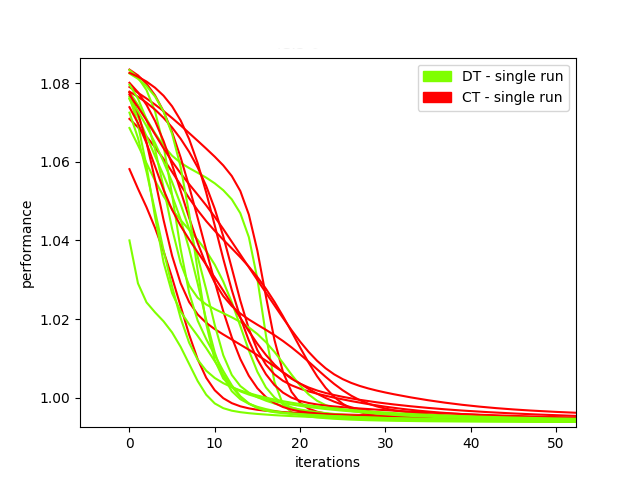
\includegraphics[width=1\linewidth]{img/ex1/1/single_runs_zoom50.png}
  \captionof{figure}{Convergence from various random starting points.}
  \label{fig:sr50}
\end{minipage}
\begin{minipage}{.8\textwidth}
  \centering
  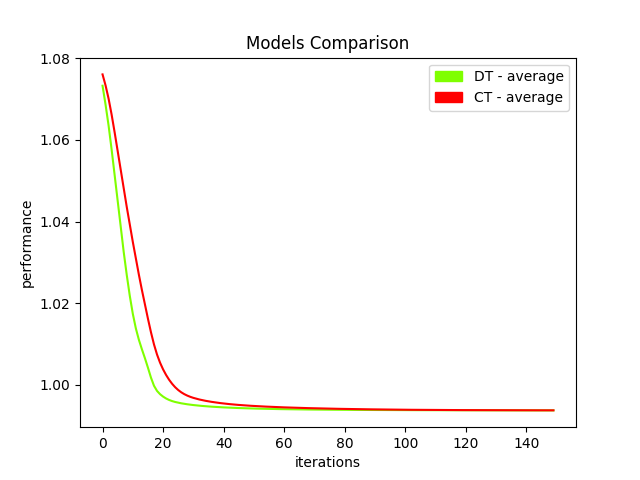
\includegraphics[width=.95\linewidth]{img/ex1/1/average.png}
  \captionof{figure}{Average convergence for various random starting points.}
  \label{fig:avgc}
\end{minipage}
\end{figure} 

\begin{figure}
\centering
\begin{minipage}{.8\textwidth}
  \centering
  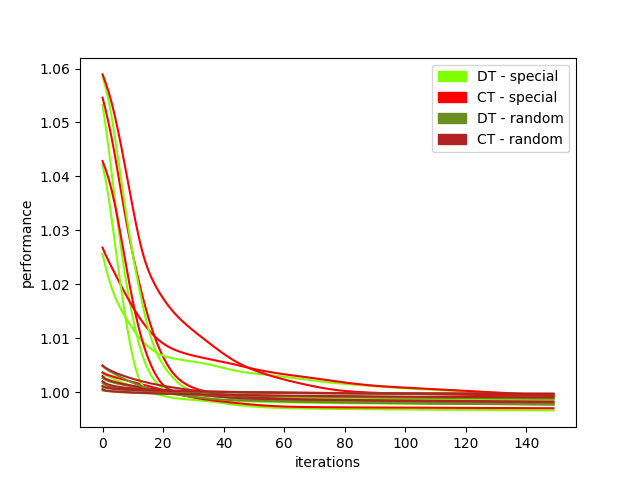
\includegraphics[width=1\linewidth]{img/ex1/2/all.png}
  \captionof{figure}{Average convergences for various generated datasets.}
  \label{fig:all}
\end{minipage}
\begin{minipage}{.8\textwidth}
  \centering
  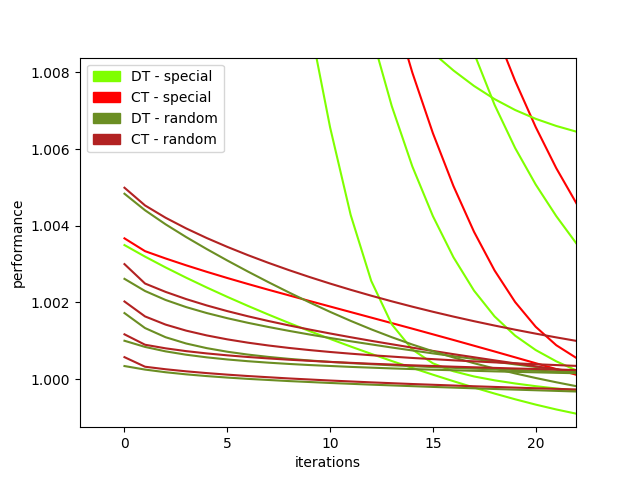
\includegraphics[width=.95\linewidth]{img/ex1/2/random.png}
  \captionof{figure}{Average convergences for various generated datasets (zoom).}
  \label{fig:random}
\end{minipage}
\end{figure}  

\item \textbf{ Conclusions }

The slower convergence of continuous-time model is caused by the different character of the model. Since in the discrete-time model we always now when the change of the state can happen (at observation), in continuous-time model it can happen in any time in between as well. Thus, while computing the new parameters during maximization step, we need to care about more unknown. In continuous-time model in-between the observation points, the probability of being in the concrete state is leading to the stationary distribution of model from previous step. The more, the further from observation point we are. This create the momentum, not presented in discrete-model, that make the convergence to be slower.

In the second experiment we have showed, how the characteristic of the searched model influenced the complexity of training. The randomly generated models generate datasets with higher entropy, that are usually closer to converge in the parameter space. 

The over-performing of the original model can be seen as the over-fitting. However it is not detectable without knowledge of the original model and, if we are sure about the number of hidden states, it is not the negative characteristic. The over-performing would probably gradually disappear with growing size of the data-set. However this experiment was not conducted to measure performance of the models, but to compare speeds of its convergence. [odkaz na dalsi exp, co to robi??]

All of the training conducted during this experiment, more or less converged to something, what seems to be global optima. We have used the simple 3-states models, the behavior of more complex models will be examined later in [odkaz].    
 	
\end{itemize}

\section{Computational Complexity}\label{sec:cc}

In this section we are comparing the time performance of two CT-HMM algorithm variants, as described in implementation part [odkaz]. We have called them float and integer-interval algorithms [odkaz].
In two subsection we will manipulate either with hidden states number or maximal time interval value and watch, if the measured values correspond the theoretical expectations \ref{sec:complex}.

\subsection{Variable Hidden-States Number}

The hidden states number, referred to as $n$ is the key parameter in overall algorithm complexity. Due to the need of knowing matrix exponentials ($n^3$) for every pair of end states, it influence the time complexity by its fifth power $n^5$. The upper bound theoretical complexity dependance on $n$ is the same for both variants, however the float-algorithm counts the matrix exponential by \textit{expm} method every time, while the integer-algorithm counts it only and then use the matrix multiplication to get the individual results \ref{it:ctc}. In the experiment we will measure the times of most costly algorithm parts, and watch how big is the portion of the overall computational complexity consumed by them. 

\begin{itemize}
\item \textbf{ Description }

We have run algorithms with variable number of hidden states. To minimize the influence of other factors, we let the number of output variables to be constantly 10 and we have used always the same randomly generated dataset, with the integral times intervals generated by exponential distribution with parameter 0.5. To minimize the time measurements error, we have always run 10 iterations of algorithm and repeat the all procedure 5 times. 

To see how the size of dataset influence the time, we have conducted all the described experiment twice , once with the \textit{small} dataset - compounding 10 sequences of 10 observations and once with the \textit{big} - compounding 10 sequences of 100 observations.  

\item \textbf{ Observation }

We can observe \ref{fig:e2n}, that under set condition is the float-interval algorithm always slower. It is caused by the big constant of \textit{expm} method, that is as you can see, in all cases the prevalent source of the complexity. In the float-interval algorithm with the small dataset are all other parts of the algorithm almost neglectable comparing to it.

Comparing to the $expm$ are the $square and multiply$ algorithm time demands considerably smaller, taking even smaller portion of time as the single $expm$ call in the integer-interval algorithm.

The increase of the dataset size caused the larger gap among the whole algorithm time-complexity and its measured subparts - either $expm$ or the sum of $expm$ and $square and multiply$ depending on the algorithm \ref{fig:e2big}.   

\begin{figure}
\centering
\begin{subfigure}{.8\textwidth}
  \centering
  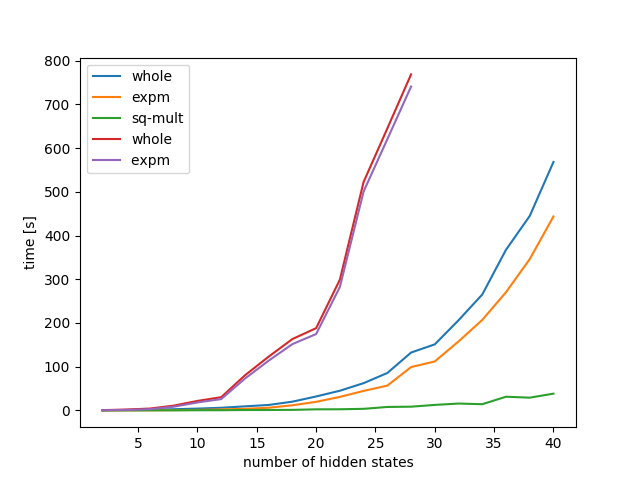
\includegraphics[width=1\linewidth]{img/ex2/small.png}
  \caption{Small dataset}
  \label{fig:e2small}
\end{subfigure}
\begin{subfigure}{.8\textwidth}
  \centering
  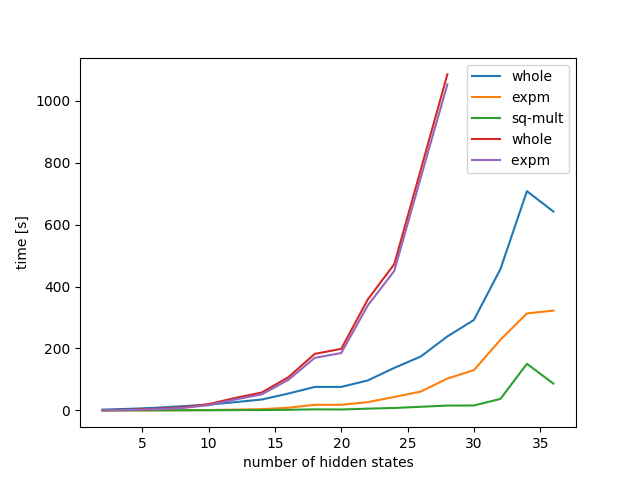
\includegraphics[width=\linewidth]{img/ex2/big.png}
  \caption{Big dataset}
  \label{fig:e2big}
\end{subfigure}
\caption{ The time-complexity of the two algorithm variants and their subparts }
\label{fig:e2n}
\end{figure}

\item \textbf{ Conclusion }

As we have only changed the number of states and let the dataset to be the same, the $max_t$ from the integer-interval complexity $\mathcal{O}(r*n^5*log(max_t))$ behaved like the constant and so, both of the algorithm have the seemingly same complexity $\mathcal{O}(r*n^5)$. The \textit{expm} method showed to have very big constant. That's way it is almost always better, if possible to use the integer-interval algorithm. (Its numerical stability is tested later in section \ref{sec:ns}) 

The most of the computational power is used to count matrix exponentials $expm$, as it is in most cases the predominant cause of algorithm "slowness", it makes not much sense to edge-optimize other parts of the algorithm. Instead, the faster implementation of $expm$, its parallelization or replacement with other method could make the thing.      

The big dataset \label{fig:e2big} has decreased the percentage of the time spent by $expm$ method in the algorithm. It is because the higher demand of other parts of the algorithm. However improbable it may be, it can possibly happen that this gap would overgrowth the $expm$ part. The $expm$ complexity is only dependent on $r$ - the number of different time intervals, however there are parts of the algorithms with complexity ${O}(n^2T)$ \ref{it:ctc}, where $T$ is number of all time intervals. So for the huge dataset with lower number of hidden states and mostly similar time intervals could this part became predominant cause of the complexity.   

\end{itemize}

\subsection{Variable Maximal Time Interval}

The other parameter present in the theoretical time-complexity of integer-interval algorithm - $\mathcal{O}(r*n^5*log(max_t))$ \ref{it:ctc} is $max_t$ - maximal length of the time interval. However it is not part of the float-interval algorithm complexity term - $\mathcal{O}(r*n^5)$. The experiment aims to observe how the variable value of $max_t$ change the computational demand of the algorithm.  

\begin{itemize}
\item \textbf{ Description }

In the experiment we have set $max_t$ as the variable, taking values of all powers of two from $2^1$ to $2^{56}$. The use of higher values (even floats) was impossible, because of conversion to 64-bites integer used in $expm$ method, that eventually caused the integer overflow. We have generated the dataset of 10 sequences of 10 observations. There were always at least one time-interval of length $max_t$ and all other were chosen uniformly from interval $[1,max_t]$. We have trained the model of $10$ hidden states and $10$ observation variables. To smooth the influence of time measurement imprecision, we have run $10$ iterations and repeat the whole experiment $5$ times.   

\item \textbf{ Observation }

Contrary to initial expectation both float and integer interval algorithm computational times are growing seemingly logarithmically with increasing $max_t$. The cause of growth in float-interval algorithm is \textit{expm} method, in integer-interval algorithm it is caused mainly by \textit{square and multiply} method. There is the steep growth of the float-interval algorithm time demand present for small $max_t$ values.

\begin{figure}[h]
\centering
\begin{minipage}{.8\textwidth}
  \centering
  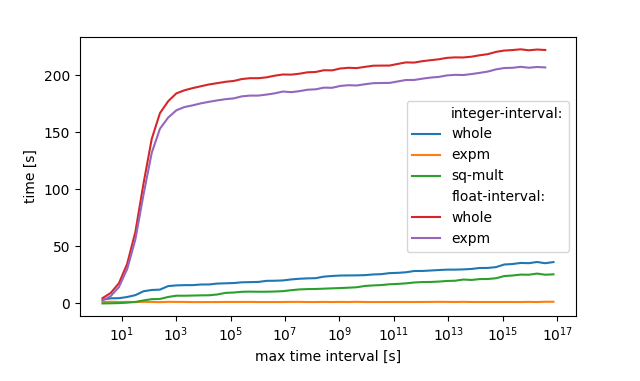
\includegraphics[width=1.0\linewidth]{img/ex2/log.png}
  \captionof{figure}{log.}
  \label{fig:e2log}
\end{minipage}
\begin{minipage}{.8\textwidth}
  \centering
  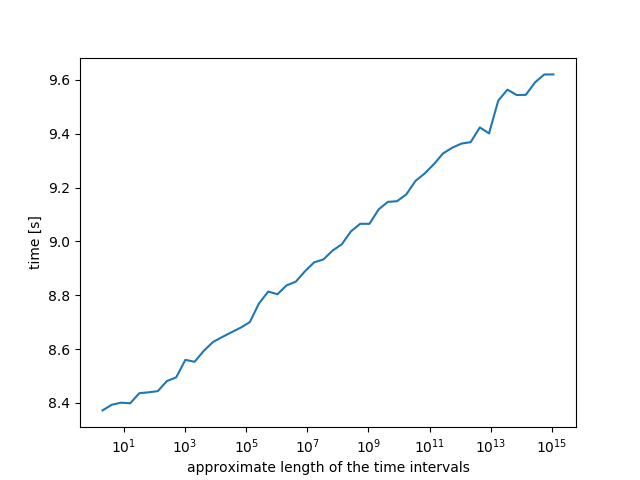
\includegraphics[width=1.0\linewidth]{img/ex2/exp180.png}
  \captionof{figure}{log2.}
  \label{fig:e2big}
\end{minipage}
\end{figure}

\item \textbf{ Conclusion }

The steep growth at the beginning is caused by choice of integral interval lengths. For small values of $max_t$ is high probability of more intervals being the same, what has direct impact at the complexity, where variable $r$ is directly present. The chance of choosing two same interval length for bigger $max_t$ values is extremely low.

The logarithmic grow of \textit{square and multiply} method is obvious. But to explain similar behavior at the $expm$ method, we need to look deeper in its implementation []%[https://github.com/scipy/scipy/blob/v0.16.1/scipy/sparse/linalg/matfuncs.py#L554]. 
The method is using Pad\'{e} approximants of different values from $3$ to $13$. The computation of the approximants of higher order is computationally more costly. The algorithm is choosing the smallest  Pad\'{e} approximant, which securely not overgrow the wished threshold error. Our observation suggest, that the bigger the numbers in the exponentiated matrix are, the bigger is the probability that the more complex Pad\'{e} approximant will be chosen.     

\end{itemize}

\begin{itemize}
\item \textbf{ Description }
\item \textbf{ Observation }
\item \textbf{ Conclusion }
\end{itemize}


\section{Numerical Stability}\label{sec:ns} 

The main advantage of integer-interval variant of algorithm is that it computes the costly matrix exponential only once and derive all other exponentials of the matrix multiplications by computing its powers, via \textit{square and multiply} method. It arise the question of numerical stability of the method. Can the inaccuracies acquired by \textit{square and multiply} change the direction of convergence?   

\begin{itemize}
\item \textbf{ Description }
In the experiment we have run both integer and float-algorithms with the same initial parameters. As the value of interest, we have measured the relative euclidean distance among both models jump-rates matrices $\matr{Q}$. We have used the models of $5$ hidden states and $5$ observable variables. At the dataset of $100$ observation points. The time intervals were generated by exponential distribution with parameter $\lambda$ equal $0.1$, $0.01$ and $0.001$ consecutively. The obtained plotted error is the average value of $10$ runs of the experiment.      

\item \textbf{ Observation }

The measured relative distance of jump-rate matrices seems to be random and it doesn't significantly increase with the growing iterations. However it seems that the variance magnitude grows with the decreasing magnitude of exponential parameter $\lambda$.   


\begin{figure}
\centering
\begin{subfigure}{.7\textwidth}
  \centering
  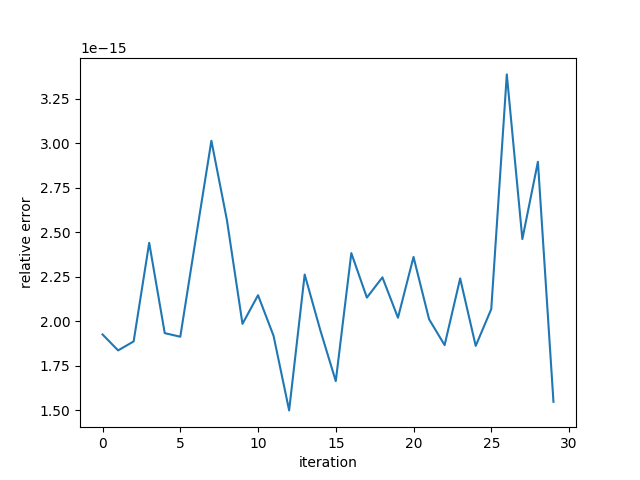
\includegraphics[width=1\linewidth]{img/ex3/relative01.png}
  \caption{ $\lambda = 0.1$ }
  \label{fig:sub1}
\end{subfigure}
\begin{subfigure}{.7\textwidth}
  \centering
  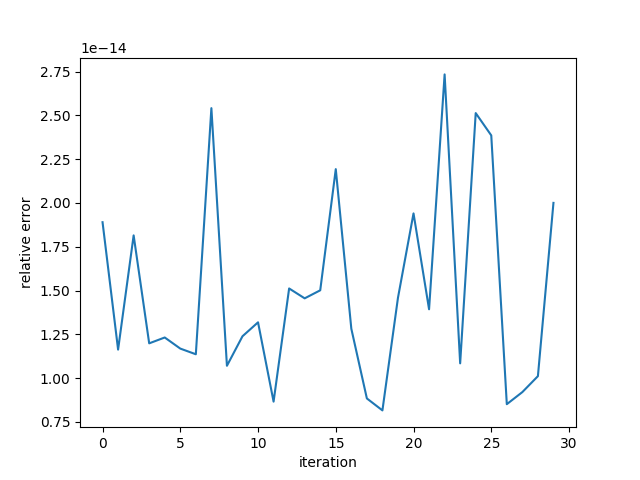
\includegraphics[width=1\linewidth]{img/ex3/relative001.png}
  \caption{$\lambda = 0.01$}
  \label{fig:sub1}
\end{subfigure}
\begin{subfigure}{.7\textwidth}
  \centering
  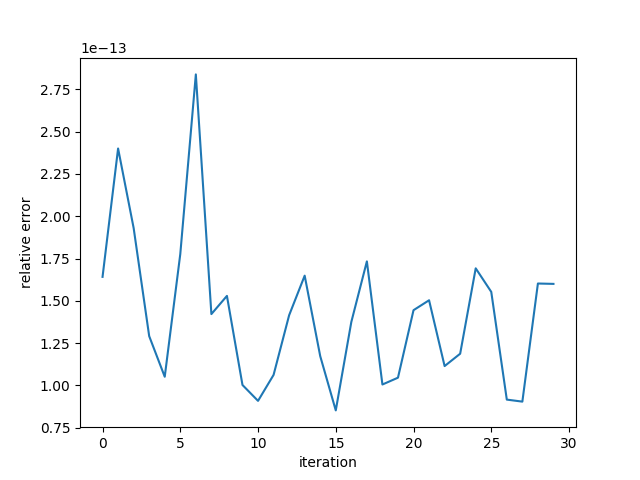
\includegraphics[width=1\linewidth]{img/ex3/relative0001.png}
  \caption{$\lambda = 0.001$}
  \label{fig:sub2}
\end{subfigure}
\caption{Relative distances of jump-rates matrices for data generated with different exponential distribution parameter $\lambda$}
\label{fig:test}
\end{figure}

\item \textbf{ Conclusion }
The experiment haven't show any error propagation trough growing iterations number. So the errors seems to be eliminated as they decrease to the local optima. It is not the proof and it is probable, that under some more extreme edge cases the matrices may diverge. However taking into account the randomness of the initial configuration and assorted characteristic of the parameter space, we do not see it as problem and we do not think it can, in general, negatively influence the performance of the algorithm.  

\end{itemize}

\section{Soft-Hard}

\begin{itemize}
\item \textbf{ Description }
\item \textbf{ Observation }

\begin{figure}
\centering
\begin{subfigure}{.8\textwidth}
  \centering
  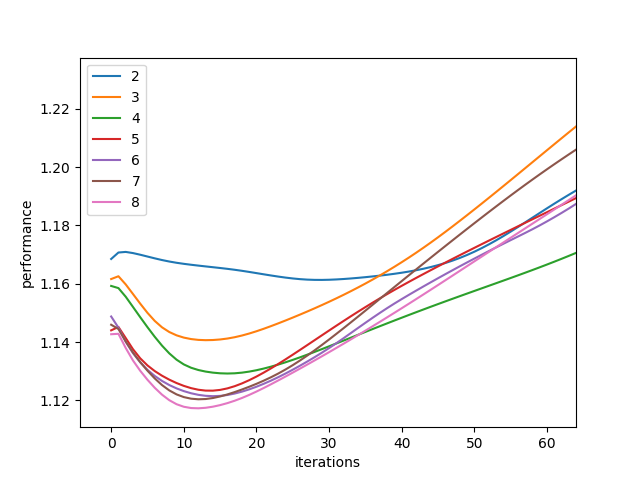
\includegraphics[width=1\linewidth]{img/ex5/test_small.png}
  \caption{A subfigure}
  \label{fig:sub1}
\end{subfigure}
\begin{subfigure}{.8\textwidth}
  \centering
  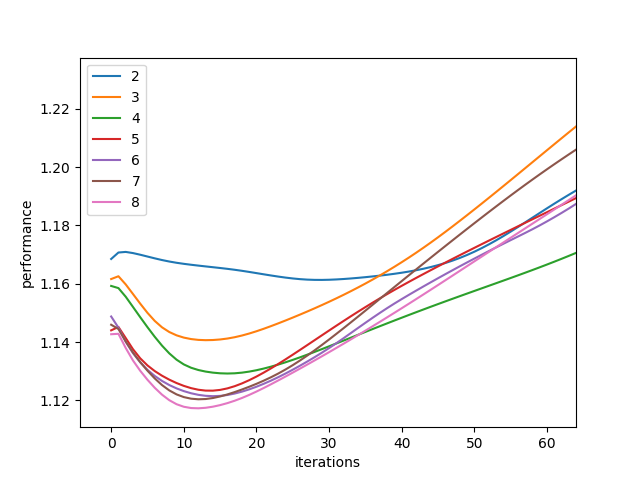
\includegraphics[width=1\linewidth]{img/ex5/test_small.png}
  \caption{A subfigure}
  \label{fig:sub2}
\end{subfigure}
\caption{A figure with two subfigures}
\label{fig:test}
\end{figure}

\begin{figure}
\centering
\begin{subfigure}{.8\textwidth}
  \centering
  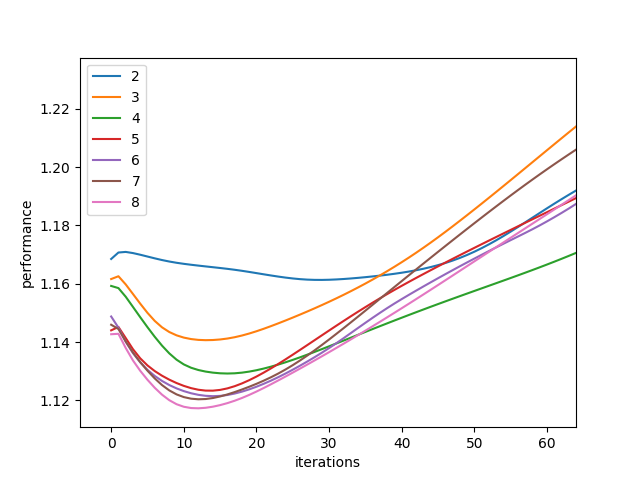
\includegraphics[width=1\linewidth]{img/ex5/test_small.png}
  \caption{A subfigure}
  \label{fig:sub1}
\end{subfigure}
\begin{subfigure}{.8\textwidth}
  \centering
  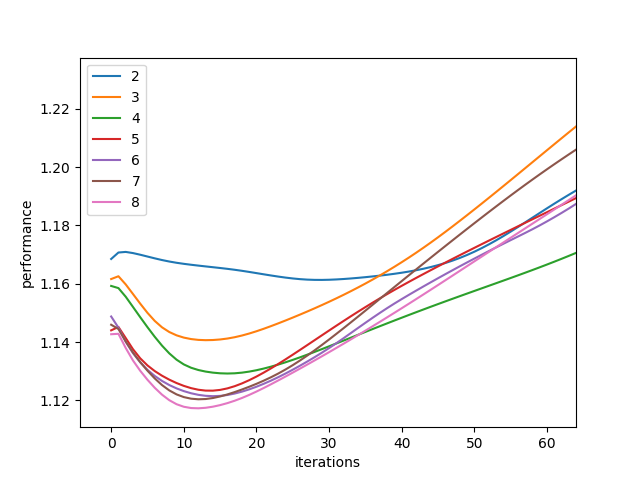
\includegraphics[width=1\linewidth]{img/ex5/test_small.png}
  \caption{A subfigure}
  \label{fig:sub2}
\end{subfigure}
\caption{A figure with two subfigures}
\label{fig:test}
\end{figure}

\item \textbf{ Conclusion }
\end{itemize}


\section{States}

\begin{itemize}
\item \textbf{ Description }
\item \textbf{ Observation }

\begin{figure}
\centering
\begin{subfigure}{.8\textwidth}
  \centering
  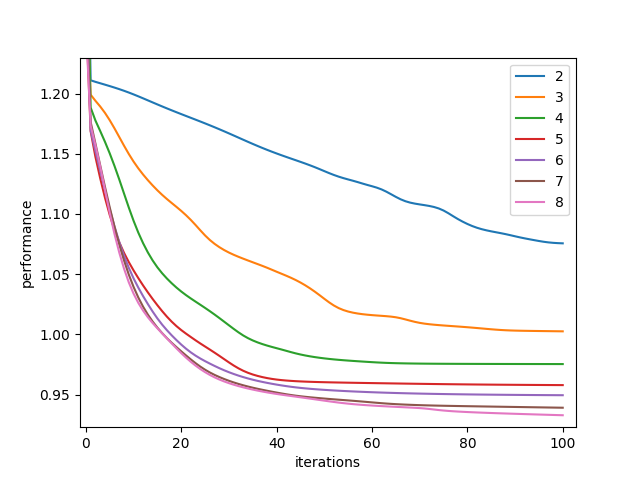
\includegraphics[width=1\linewidth]{img/ex5/train_small.png}
  \caption{A subfigure}
  \label{fig:sub1}
\end{subfigure}
\begin{subfigure}{.8\textwidth}
  \centering
  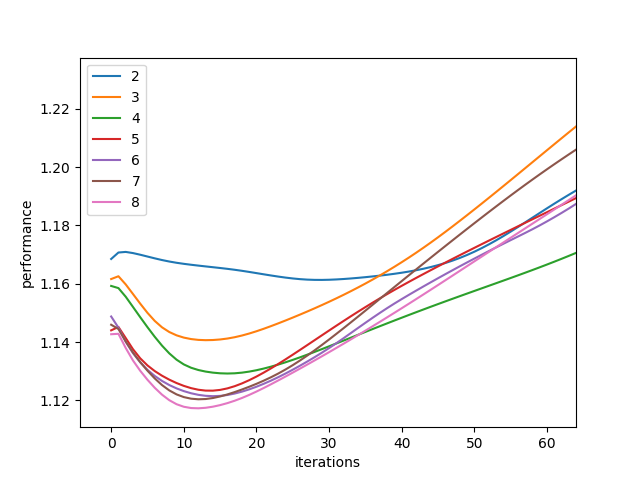
\includegraphics[width=1\linewidth]{img/ex5/test_small.png}
  \caption{A subfigure}
  \label{fig:sub2}
\end{subfigure}
\caption{A figure with two subfigures}
\label{fig:test}
\end{figure}

\begin{figure}
\centering
\begin{subfigure}{.8\textwidth}
  \centering
  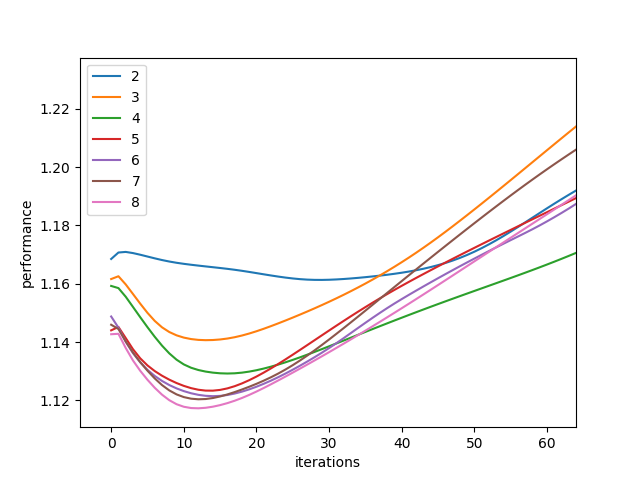
\includegraphics[width=1\linewidth]{img/ex5/test_small.png}
  \caption{A subfigure}
  \label{fig:sub1}
\end{subfigure}
\begin{subfigure}{.8\textwidth}
  \centering
  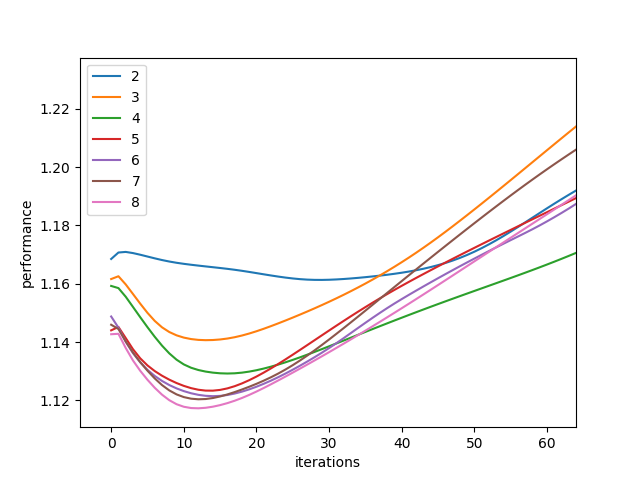
\includegraphics[width=1\linewidth]{img/ex5/test_small.png}
  \caption{A subfigure}
  \label{fig:sub2}
\end{subfigure}
\caption{A figure with two subfigures}
\label{fig:test}
\end{figure}

\item \textbf{ Conclusion }
\end{itemize}


%\chapter{EM Algorithms for CT-HMM}


% expm reference form scipy: The Scaling and Squaring Method for the Matrix Exponential Revisited",
%    SIAM. J. Matrix Anal. & Appl. 26, 1179 (2005).

%http://mathoverflow.net/questions/239073/what-is-the-time-complexity-of-the-matrix-exponential/239083


%\chapter{Realisation}

\setsecnumdepth{part}
\chapter{Conclusion}

malo informacie (vela hidden) menej presny.
rychlo sa straca informacia 

\section{Future Work}


\bibliographystyle{iso690}
\bibliography{mybibliographyfile}

\setsecnumdepth{all}
\appendix

\chapter{Acronyms}
% \printglossaries
\begin{description}
	\item[DTMC] Discrete-time Markov Chain	
	\item[CTMC] Continuous-time Markov Chain
	\item[DT-HMM] Discrete-time Hidden Markov Model
	\item[CT-HMM] Continuous-time Hidden Markov Model
	\item[EM] Expectation-Maximization 
	\item[MLE] Maximum likelihood estimation
\end{description}


\chapter{Contents of enclosed CD}

%change appropriately

\begin{figure}
	\dirtree{%
		.1 readme.txt\DTcomment{the file with CD contents description}.
		.1 exe\DTcomment{the directory with executables}.
		.1 src\DTcomment{the directory of source codes}.
		.2 wbdcm\DTcomment{implementation sources}.
		.2 thesis\DTcomment{the directory of \LaTeX{} source codes of the thesis}.
		.1 text\DTcomment{the thesis text directory}.
		.2 thesis.pdf\DTcomment{the thesis text in PDF format}.
		.2 thesis.ps\DTcomment{the thesis text in PS format}.
	}
\end{figure}

\end{document}
